%%
%% This is file `sigconf.tex',
%% generated with the docstrip utility.
%%
%% The original source files were:
%%
%% samples.dtx  (with options: `all,proceedings,sigconf')
%% 
%% IMPORTANT NOTICE:
%% 
%% For the copyright see the source file.
%% 
%% Any modified versions of this file must be renamed
%% with new filenames distinct from sigconf.tex.
%% 
%% For distribution of the original source see the terms
%% for copying and modification in the file samples.dtx.
%% 
%% This generated file may be distributed as long as the
%% original source files, as listed above, are part of the
%% same distribution. (The sources need not necessarily be
%% in the same archive or directory.)
%%
%%
%% Commands for TeXCount
%TC:macro \cite [option:text,text]
%TC:macro \citep [option:text,text]
%TC:macro \citet [option:text,text]
%TC:envir table 0 1
%TC:envir table* 0 1
%TC:envir tabular [ignore] word
%TC:envir displaymath 0 word
%TC:envir math 0 word
%TC:envir comment 0 0
%%
%% The first command in your LaTeX source must be the \documentclass
%% command.
%%
%% For submission and review of your manuscript please change the
%% command to \documentclass[manuscript, screen, review]{acmart}.
%%
%% When submitting camera ready or to TAPS, please change the command
%% to \documentclass[sigconf]{acmart} or whichever template is required
%% for your publication.
%%
%%
% \documentclass[sigconf]{acmart}
\documentclass[sigconf, anonymous, review]{acmart}
%%
%% \BibTeX command to typeset BibTeX logo in the docs
\AtBeginDocument{%
  \providecommand\BibTeX{{%
    Bib\TeX}}}

%% Rights management information.  This information is sent to you
%% when you complete the rights form.  These commands have SAMPLE
%% values in them; it is your responsibility as an author to replace
%% the commands and values with those provided to you when you
%% complete the rights form.
\setcopyright{acmlicensed}
\copyrightyear{2018}
\acmYear{2018}
\acmDOI{XXXXXXX.XXXXXXX}
%% These commands are for a PROCEEDINGS abstract or paper.
\acmConference[Conference acronym 'XX]{Make sure to enter the correct
  conference title from your rights confirmation email}{June 03--05,
  2018}{Woodstock, NY}
%%
%%  Uncomment \acmBooktitle if the title of the proceedings is different
%%  from ``Proceedings of ...''!
%%
%%\acmBooktitle{Woodstock '18: ACM Symposium on Neural Gaze Detection,
%%  June 03--05, 2018, Woodstock, NY}
\acmISBN{978-1-4503-XXXX-X/2018/06}


%%
%% Submission ID.
%% Use this when submitting an article to a sponsored event. You'll
%% receive a unique submission ID from the organizers
%% of the event, and this ID should be used as the parameter to this command.
%%\acmSubmissionID{123-A56-BU3}

%%
%% For managing citations, it is recommended to use bibliography
%% files in BibTeX format.
%%
%% You can then either use BibTeX with the ACM-Reference-Format style,
%% or BibLaTeX with the acmnumeric or acmauthoryear sytles, that include
%% support for advanced citation of software artefact from the
%% biblatex-software package, also separately available on CTAN.
%%
%% Look at the sample-*-biblatex.tex files for templates showcasing
%% the biblatex styles.
%%
%%
%% The majority of ACM publications use numbered citations and
%% references.  The command \citestyle{authoryear} switches to the
%% "author year" style.
%%
%% If you are preparing content for an event
%% sponsored by ACM SIGGRAPH, you must use the "author year" style of
%% citations and references.
%% Uncommenting
%% the next command will enable that style.
%%\citestyle{acmauthoryear}


%%
%% end of the preamble, start of the body of the document source.
\begin{document}

%%
%% The "title" command has an optional parameter,
%% allowing the author to define a "short title" to be used in page headers.
\title{When Minority Opinions Become Dissent: How Online Crowds Punish and Engage Challenges to Moral Consensus}

%%
%% The "author" command and its associated commands are used to define
%% the authors and their affiliations.
%% Of note is the shared affiliation of the first two authors, and the
%% "authornote" and "authornotemark" commands
%% used to denote shared contribution to the research.
\author{Ben Trovato}
\authornote{Both authors contributed equally to this research.}
\email{trovato@corporation.com}
\orcid{1234-5678-9012}
\author{G.K.M. Tobin}
\correspondingauthor
\authornotemark[1]
\email{webmaster@marysville-ohio.com}
\affiliation{%
  \institution{Institute for Clarity in Documentation}
  \city{Dublin}
  \state{Ohio}
  \country{USA}
}

\author{Lars Th{\o}rv{\"a}ld}
\affiliation{%
  \institution{The Th{\o}rv{\"a}ld Group}
  \city{Hekla}
  \country{Iceland}}
\email{larst@affiliation.org}

\author{Valerie B\'eranger}
\affiliation{%
  \institution{Inria Paris-Rocquencourt}
  \city{Rocquencourt}
  \country{France}
}

\author{Aparna Patel}
\affiliation{%
 \institution{Rajiv Gandhi University}
 \city{Doimukh}
 \state{Arunachal Pradesh}
 \country{India}}

\author{Huifen Chan}
\affiliation{%
  \institution{Tsinghua University}
  \city{Haidian Qu}
  \state{Beijing Shi}
  \country{China}}

\author{Charles Palmer}
\affiliation{%
  \institution{Palmer Research Laboratories}
  \city{San Antonio}
  \state{Texas}
  \country{USA}}
\email{cpalmer@prl.com}

\author{John Smith}
\affiliation{%
  \institution{The Th{\o}rv{\"a}ld Group}
  \city{Hekla}
  \country{Iceland}}
\email{jsmith@affiliation.org}

\author{Julius P. Kumquat}
\correspondingauthor
\affiliation{%
  \institution{The Kumquat Consortium}
  \city{New York}
  \country{USA}}
\email{jpkumquat@consortium.net}

%%
%% By default, the full list of authors will be used in the page
%% headers. Often, this list is too long, and will overlap
%% other information printed in the page headers. This command allows
%% the author to define a more concise list
%% of authors' names for this purpose.
\renewcommand{\shortauthors}{Trovato et al.}

%%
%% The abstract is a short summary of the work to be presented in the
%% article.
\begin{abstract}
Minority moral judgments can assign blame to someone the crowd absolves or defend someone the crowd blames. How do these directions of dissent differ in their reception, and how does minority expression develop across communities? We analyze more than 15 million top-level judgment comments from r/AmItheAsshole (AITA) and r/AITAH (AITAH), combining voting and reply measures with annotations of expressed linguistic certainty and comparisons of matched stories. We distinguish high-agreement posts, where at least 80\% of judgments favor one side, from low-agreement posts, where judgments are split 40–60\%. Majority–minority differences in scores and reply engagement are larger in high-agreement posts. Within these posts, both blaming and defending minority judgments receive lower scores but greater reply engagement than majority judgments in their respective judgment contexts. The score–reply pattern thus recurs in both directions of dissent and both communities, but its magnitude is asymmetric: blaming minority judgments receive lower mean scores and attract more replies and deeper reply trees than defending minority judgments. Minority certainty rises over the observed window in AITA, while no significant overall trend is detected in AITAH. The cumulative share of defending minority judgments increases slightly in AITA but declines in AITAH. Matched stories also exhibit a larger majority–minority score gap in AITA. These observational comparisons do not isolate the effect of AITA’s official verdict flair. Together, the findings establish a shared reception pattern across opposing moral judgments while revealing directional asymmetries and community-specific patterns in minority expression over time.
\end{abstract}

%%
%% The code below is generated by the tool at http://dl.acm.org/ccs.cfm.
%% Please copy and paste the code instead of the example below.
%%
\begin{CCSXML}
<ccs2012>
 <concept>
  <concept_id>00000000.0000000.0000000</concept_id>
  <concept_desc>Do Not Use This Code, Generate the Correct Terms for Your Paper</concept_desc>
  <concept_significance>500</concept_significance>
 </concept>
 <concept>
  <concept_id>00000000.00000000.00000000</concept_id>
  <concept_desc>Do Not Use This Code, Generate the Correct Terms for Your Paper</concept_desc>
  <concept_significance>300</concept_significance>
 </concept>
 <concept>
  <concept_id>00000000.00000000.00000000</concept_id>
  <concept_desc>Do Not Use This Code, Generate the Correct Terms for Your Paper</concept_desc>
  <concept_significance>100</concept_significance>
 </concept>
 <concept>
  <concept_id>00000000.00000000.00000000</concept_id>
  <concept_desc>Do Not Use This Code, Generate the Correct Terms for Your Paper</concept_desc>
  <concept_significance>100</concept_significance>
 </concept>
</ccs2012>
\end{CCSXML}

\ccsdesc[500]{Do Not Use This Code~Generate the Correct Terms for Your Paper}
\ccsdesc[300]{Do Not Use This Code~Generate the Correct Terms for Your Paper}
\ccsdesc{Do Not Use This Code~Generate the Correct Terms for Your Paper}
\ccsdesc[100]{Do Not Use This Code~Generate the Correct Terms for Your Paper}

%%
%% Keywords. The author(s) should pick words that accurately describe
%% the work being presented. Separate the keywords with commas.
\keywords{Do, Not, Use, This, Code, Put, the, Correct, Terms, for,
  Your, Paper}
%% A "teaser" image appears between the author and affiliation
%% information and the body of the document, and typically spans the
%% page.
% \begin{teaserfigure}
%  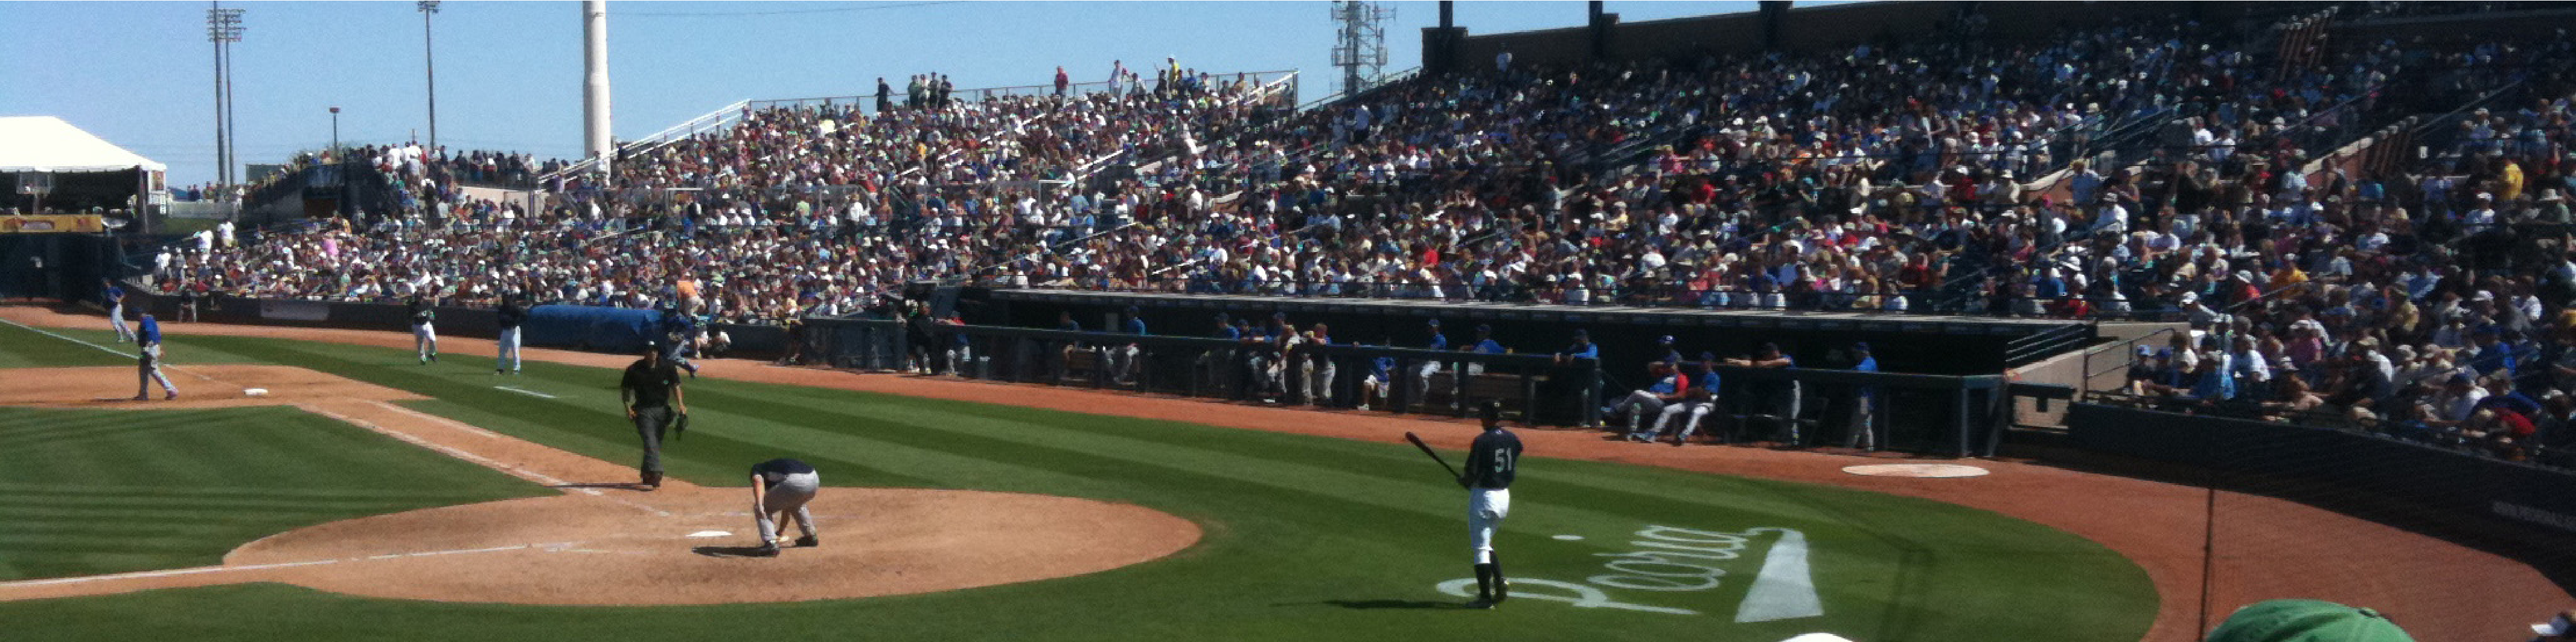
\includegraphics[width=\textwidth]{sampleteaser}
%   \caption{Seattle Mariners at Spring Training, 2010.}
%   \Description{Enjoying the baseball game from the third-base
%   seats. Ichiro Suzuki preparing to bat.}
%   \label{fig:teaser}
% \end{teaserfigure}

\received{20 February 2007}
\received[revised]{12 March 2009}
\received[accepted]{5 June 2009}

%%
%% This command processes the author and affiliation and title
%% information and builds the first part of the formatted document.
\maketitle


\section{Introduction}
\label{sec:intro}

% Paragraph 1: Motivate the stakes of blaming and defending as two directions of dissent.
When online communities judge everyday interpersonal conflicts, the majority's verdict is not the only perspective at stake. A dissenting judgment can call for accountability where others see no wrongdoing, or question condemnation that others accept. How these judgments are received matters for understanding whether a discussion accommodates challenges to both collective blame and collective defense. Neither kind of dissent is necessarily correct, but treating them as interchangeable obscures which challenges attract approval, opposition, or sustained conversation. We therefore focus on minority judgments about whether someone is at fault, distinguishing \emph{blaming dissent}, which assigns fault to someone whom most others defend, from \emph{defending dissent}, which rejects fault assigned by most others. Does the direction of dissent shape how others respond and how minority judgments develop over time?

% Paragraph 2: Establish alignment and agreement strength as the context for dissent.
Understanding this distinction requires situating each judgment within the surrounding distribution of opinion. A blaming judgment can express the majority position in one discussion and constitute a minority position in another. The strength of agreement also matters: opposing a narrow majority in a divided discussion differs from challenging a judgment that nearly everyone else supports. We therefore distinguish \emph{majority} from \emph{minority} judgments, and \emph{high-agreement} from \emph{low-agreement} posts. Our primary focus is minority dissent in high-agreement posts, where one judgment strongly predominates. These discussions make the question particularly salient: an overwhelming majority can coexist with continuing disagreement, and the final verdict alone tells us little about how that disagreement is treated or expressed. Low-agreement posts provide a comparison condition for interpreting this experience, rather than an equivalent setting of dissent against a strong majority.

% Paragraph 3: Use prior work and the spiral of silence to motivate the research gap.
Prior research provides important foundations for studying this experience. Work on Reddit shows that negative evaluations can coexist with attention through replies \cite{davis2021emotional}, while research on moral-judgment discussions examines how the value placed on agreement and dissent varies with consensus strength \cite{mellody2025consensus}. We revisit majority--minority differences in scores and conversational engagement across agreement levels as an empirical baseline, rather than treating their reappearance as a new research question. Our central question is what this aggregate comparison can conceal: whether the reception of dissent differs according to whether it blames or defends the person under judgment.

The spiral of silence further motivates examining minority participation alongside its reception. This account links perceptions of an unfavorable opinion climate to reluctance to speak out, through concern about social isolation \cite{noelleneumann1974spiral}. It directs attention to whether minority judgments continue to appear as a discussion unfolds, without implying that all dissent must steadily disappear. Our observational data capture public comments, not unspoken opinions, perceived isolation, or individual willingness to speak. We therefore examine changes in the prevalence of expressed minority judgments, rather than treating them as direct measurements of silence or self-censorship.

% Paragraph 4: Introduce AITA, the baseline, and the two primary research questions.
We investigate these questions primarily in r/AmItheAsshole (AITA), where an original poster (OP) describes an interpersonal situation and commenters judge the OP's conduct using tags such as YTA (``You're the Asshole'') and NTA (``Not the Asshole''). These explicit verdicts allow us to identify minority judgments relative to each post's dominant position and distinguish blaming from defending dissent. Section~\ref{subsec:method} defines the verdict grouping, alignment labels, and agreement thresholds; Appendix~\ref{sec:appendix-tags} explains the other verdict tags and variants.

After establishing the majority--minority baseline, we ask:

\begin{description}
    \item[\textbf{RQ1: Reception.}] Within high-agreement posts, how do blaming and defending dissent differ in the evaluations and conversational responses they receive?
    \item[\textbf{RQ2: Temporal dynamics.}] How does the prevalence of blaming and defending dissent change as discussions unfold in high-agreement posts?
\end{description}

% Paragraph 5: Introduce AITAH as a subsequent extension, not an institutional experiment.
We then extend the analysis to r/AITAH (AITAH), another community devoted to interpersonal moral judgment, to examine which patterns recur and which differ in another community context:

\begin{description}
    \item[\textbf{RQ3: Community context.}] Which patterns in the reception and temporal prevalence of blaming and defending dissent recur in AITAH, and which differ?
\end{description}

This comparison broadens the empirical scope without assuming that the two communities follow the same trajectory. It does not isolate the effects of any particular moderation practice or verdict rule.

% Paragraph 6: Summarize evidence and contributions without elevating baseline replication.
Our analyses combine comment scores and reply structure with annotations of direct replies. We separate OP replies from those of other commenters when examining challenge, allowing us to characterize responses beyond the person whose conduct is under judgment. The reception analyses distinguish the familiar majority--minority score--reply pattern from differences between the two directions of dissent: blaming minority judgments receive lower mean scores and greater reply engagement than defending minority judgments, while annotated replies show that minority judgments attract more challenge than majority judgments across the analyzed strata. The temporal analyses examine minority share, distinguishing cumulative prevalence from the composition of comments arriving in successive time windows. A supplementary annotation analysis compares expressed linguistic certainty across dissent directions over the full observed period, separately from RQ2. The AITAH extension examines whether reception and participation patterns recur in another community.

The central contribution is a direction-sensitive account of minority moral dissent: we distinguish challenging a crowd's defense of someone from challenging its condemnation, and examine both the reception of these positions and their prevalence as discussions unfold. The community extension identifies shared reception patterns alongside variation in participation. Together, these analyses show why understanding minority voices requires attention to what their disagreement does in a particular moral discussion, rather than treating all opposition to the majority as a single experience.

\section{Related Work}
\label{sec:related-work}

\subsection{Consensus Strength and Minority Dissent}

Classic research on social influence shows that disagreement with a group is not equivalent across opinion climates. A unanimous majority can alter even judgments about relatively unambiguous stimuli \cite{asch1956independence}, through both normative pressure to avoid social rejection and informational reliance on others \cite{deutsch1955normative}. More directly, the influence of majority and minority sources varies with the level of consensus surrounding their positions \cite{martin2002consensus}, and meta-analytic evidence indicates that smaller deviant factions face stronger rejection \cite{tata1996proportionate}. These findings motivate treating consensus strength as a substantive moderator rather than merely a descriptive property of a thread. Accordingly, we distinguish high-agreement posts, in which YA or NA judgments constitute at least 80\% of verdict-bearing comments, from low-agreement posts, in which the two judgment classes each constitute roughly half. Throughout, \emph{minority} denotes a numerical minority of expressed judgments within a post, rather than a demographic minority or an enduring identity group.

Research on reactions to deviants further suggests that negative evaluation and communication can coexist. In Schachter's foundational study, groups directed communication toward a deviant member in an effort to restore uniformity, yet ultimately rejected the deviant when disagreement persisted \cite{schachter1951deviation}. A later replication recovered the rejection effect but found weaker evidence for concentrated communication \cite{wesselmann2014revisiting}, underscoring the need to test these processes in other settings. Subsequent work has similarly characterized dissent as both a threat to group uniformity and a potential resource for group functioning \cite{jetten2014deviance}. Minority views can promote divergent processing \cite{nemeth1986differential}, exert indirect influence despite limited public acceptance \cite{wood1994minority}, and increase a group's cognitive complexity even while their advocates are socially rejected \cite{curseu2012socially}. This literature therefore anticipates a possible tension between the social cost borne by dissenters and the conversation their dissent generates. It has not, however, established how that tension varies between strong and divided consensus in large, naturally occurring online moral discussions.

\subsection{Evaluative Sanction and Conversational Engagement Online}

On social platforms, votes are not passive measurements of independent preferences. Early ratings can causally shape later evaluations \cite{muchnik2013social,glenski2017rating}, and negative community feedback can influence users' subsequent production and evaluation behavior \cite{cheng2014community}. On Reddit in particular, voting simultaneously expresses evaluation, enforces local norms, and affects content ranking and visibility \cite{graham2021sociomateriality}. A comment's final score should thus be understood as a socially and technologically mediated evaluative outcome, rather than a direct count of agreement alone.

Evaluative and conversational responses also capture different forms of engagement. Likes, shares, and comments respond to different content properties and should not be collapsed into a single engagement construct \cite{tenenboim2022comments}. Likewise, replying, disliking, and flagging are behaviorally distinct reactions to objectionable comments \cite{kalch2017replying}, and disagreement can attract attention without producing endorsement or sharing \cite{dutceac2022cueing}. Most directly, Davis and Graham show that downvoted Reddit comments can receive more direct replies and larger reply trees than comparable upvoted comments, describing the combination as an ``attention reward'' accompanying the emotional cost of negative ratings \cite{davis2021emotional}. Our study builds on this result but changes the inferential target: rather than using a low score as a proxy for norm deviation, we identify whether a comment's substantive moral judgment agrees with the dominant judgment of its post. This permits us to test whether the sanction--engagement split is specific to dissent under strong consensus, whether it remains under divided judgment, and whether minority status primarily affects entry into a reply exchange or its subsequent escalation. We additionally evaluate the aggregate score of the resulting subtree, while treating this measure as reception of the conversation rather than evidence of deliberative quality.

Research on controversy provides a complementary, thread-level perspective. Controversy can increase conversational interest while also creating discomfort, producing a non-monotonic relationship with discussion \cite{chen2013controversy}. On Reddit, mixed positive and negative feedback and the structure of early replies can predict whether a post will become controversial \cite{hessel2019brewing}. These definitions concern controversy around an item, whereas our comparison concerns the distribution of explicit YA and NA judgments and the relative treatment of speakers within the same thread. Prior studies of conversation trees further show that a large thread can arise either from broad one-time participation or from repeated exchanges among a smaller set of users \cite{backstrom2013threads,choi2015reddit}. This distinction motivates our separation of reply entry from escalation: a minority comment may be unusually likely to trigger a confrontation without changing how far an exchange develops once one has begun.

\subsection{Moralized Dissent, Certainty, and Selective Expression}

Moral disagreement may intensify these dynamics because negative and positive moral evaluations are not simple mirror images. Blame tends to be more differentiated and, in many settings, more extreme than praise \cite{guglielmo2019asymmetric}; proscriptive morality also places stricter demands on avoiding wrongdoing than prescriptive morality places on performing good actions \cite{janoffbulman2009proscriptive}. Blame is therefore not only a private assessment but also a communicative act that identifies and regulates perceived norm violations \cite{malle2014blame}. Online, moral-emotional language is associated with greater diffusion \cite{brady2017emotion}, and social feedback can reinforce subsequent expressions of moral outrage \cite{brady2021social}. These accounts motivate our comparison between \emph{blaming dissent} (a minority YA judgment in an NA-dominant post) and \emph{defending dissent} (a minority NA judgment in a YA-dominant post). We do not equate defense with praise; rather, the blame literature motivates the narrower hypothesis that oppositely directed moral judgments need not provoke symmetric responses.

Opinion-climate research also predicts selection in who voices dissent and how dissent is expressed. The spiral-of-silence tradition argues that perceiving oneself to be in the minority can inhibit public expression \cite{noelleneumann1974spiral}. Experiments in online forums likewise find selective posting in response to the surrounding opinion climate \cite{yun2011selective}, while anticipated personal attacks and rejection can suppress minority expression in both online and offline settings \cite{neubaum2018sanctions}. Importantly, such inhibition is heterogeneous: people with greater attitude certainty are more willing to express minority positions in unfavorable climates \cite{matthes2010spiral}. Social consensus can itself affect certainty, although its direction depends on whether belonging or distinctiveness is salient \cite{clarkson2013consensus}, and doubtful language receives fewer recommendations than confident language in large-scale online discussions \cite{evans2023doubt}.

These studies inform, but do not identify, the mechanism behind temporal changes in our data. Because Reddit traces reveal expressed comments rather than unspoken opinions, increasing certainty among later minority comments may reflect selective entry or persistence by highly committed dissenters, within-person attitude strengthening, or both. We therefore describe our annotation as \emph{expressed linguistic certainty}, not latent attitude certainty, and interpret temporal changes as compositional patterns consistent with selective expression rather than direct evidence of individual persuasion.

\subsection{Collective Moral Judgment and Institutionalized Consensus in AITA Communities}

AITA has become an important setting for studying everyday morality because it combines first-person narratives, explicit categorical judgments, voting, and threaded discussion. Nguyen et al. \cite{nguyen2022mapping} mapped more than 100,000 AITA dilemmas into fine-grained topics and related those topics to aggregate YA and NA verdicts. Subsequent research has expanded the empirical map of everyday dilemma types and their aggregate evaluations \cite{yudkin2025large}, examined the situational organization of moral disagreement \cite{shi2025moral}, and analyzed demographic variation in AITA judgments as expressions of social norms \cite{decandia2022socialnorms}. Other studies focus on how narrative features relate to verdicts \cite{giorgi2023author} and on the moral rationales expressed in judgment comments \cite{xi2024morality}. Collectively, this literature has primarily asked what kinds of dilemmas appear, how they are narrated and justified, and which collective verdict they receive. We instead shift the unit of analysis to the unequal reception of individual comments that compose---and contest---the collective verdict.

Three recent studies are especially close to our analysis. Mellody models how agreement and dissent are valued as a consensus develops in AITA, finding that the association between dissent and comment score varies with consensus strength \cite{mellody2025consensus}. Its primary analysis restricts the sample to comments with scores of at least one, following the community's stated rule that downvotes should indicate irrelevance; negatively evaluated comments therefore lie outside its principal estimand. Our analysis retains zero and negative scores because evaluative suppression is itself an outcome of interest, and it jointly examines replies, depth, subtree reception, moral direction, expressed certainty, and time. Goglia and Vega model AITA threads as growing interaction networks and relate thread-level disagreement to their structural evolution \cite{goglia2024structure}; our focus is instead which stance attracts replies within a thread and whether minority status affects conversational entry or escalation. Finally, Goglia, Vega, and Gandelli analyze judgment composition and language before and after AITA's 18-hour verdict disclosure \cite{goglia2026influence}. They report post-disclosure shifts but explicitly caution that self-selection and algorithmic visibility preclude a causal interpretation. Consistent with that caution, we distinguish gradual temporal trends from any discontinuity at 18 hours and interpret a post-lock coefficient as a conditional association rather than a verdict effect.

The comparison between AITA and AITAH provides an institutional boundary condition rather than a natural experiment. Subreddit rules and governance can shape participation and local norms \cite{fiesler2018rules}, and even making community rules more salient can change newcomer participation and compliance \cite{matias2019norms}. AITA and AITAH differ not only in whether a formal verdict is assigned after 18 hours but also in size, moderation, membership, and other unobserved characteristics. We therefore use AITAH to test replication under a community without the formal verdict rule, not to identify the causal effect of flair assignment. Bringing these literatures together, our study asks when numerical dissent becomes a locally deviant voice and traces its reception across four distinct channels---evaluation, conversation, language, and time---while using moral direction and institutional context to characterize where the pattern varies.

\section{Data and Methods}
\label{sec:data-method}

\subsection{Data Sources and Analytical Samples}
\label{subsec:dataset}

We study everyday moral judgments in r/AmItheAsshole (AITA), where an
original poster (OP) describes an interpersonal situation and commenters
judge the OP's conduct. We extend the analysis to r/AITAH (AITAH), which
supports a similar narrative-and-judgment format and verdict vocabulary.
AITA is the primary setting; AITAH provides a second community context in
which to examine the reception and expression of blaming and defending dissent.

We use archived public submissions and comments covering 2018--2025.
\textbf{[TODO: identify the archive source, provide its citation, and report
retrieval dates and known coverage limitations.]}
Within-community analyses use the available observations for each community.
Direct cross-community comparisons use the common period from 17 March 2021
to 23 December 2025. For each eligible verdict comment, we retain its post
identifier, text, verdict group, score, timestamp, and links to its replies.

\paragraph{Eligibility and coverage.}
Our judgment-level unit is a top-level verdict comment: a direct reply to a
submission whose extracted label belongs to a retained verdict group. The main analyses include posts
with at least $200$ retained verdict comments and exclude exact ties between
YA and NA, as defined below. Nested replies are analyzed as responses to
judgments rather than included in the post's verdict distribution.
\textbf{[TODO: specify treatment of deleted text, bots, and unavailable authors;
report counts before and after filtering by community.]}

Comment-count and score analyses use all eligible observations in the
collected dataset. This describes coverage of retained archive data, not
complete coverage of community activity. Reply depth and subtree score use a
random sample of posts because they require recursive reply-tree traversal.
Language analyses use separate annotated samples, not annotations of the full
dataset. Certainty annotation concerns top-level comments attached to sampled
posts with at least $200$ retained YA/NA verdict comments
($\mathrm{YANA\_total}\ge200$), rather than a single label for each post.
The sampling plan supplements earlier annotations toward coverage of $3\%$
of eligible high-agreement posts and $15\%$ of eligible low-agreement posts.
The certainty-annotated dataset used in this paper comprises $1{,}195$
low- and high-agreement posts. Intermediate-agreement posts present in the
broader annotation file are excluded from this dataset. Posts are the
sampling unit and comments the annotation unit; these annotations do not
cover the full collected dataset.

The $1{,}195$ posts include five exact-tie AITA posts under the stored
final-verdict metadata, which are excluded from directional comparisons.
The full-observed-period certainty analysis below further requires an observed
minority comment with a valid certainty label and includes $1{,}169$
contributing posts and $104{,}135$ minority comments. These analysis-specific
counts are distinct from the size of the annotated dataset.
\textbf{[TODO: reconcile the within-dataset breakdown: the stored metadata
give AITA 659/276 and AITAH 202/58 high/low posts, whereas the previously
reported counts are AITA 659/277 and AITAH 201/58; both total 1,195.
Document the sampling history and final-verdict metadata version. Report
completed annotation counts for the 1,195-post low/high dataset, separately
from retained analysis comments; do not use comment totals from the broader
annotation file or infer population sampling weights from nominal fractions.]}

Direct-response annotation uses three samples of $16{,}000$ parent--reply
pairs each, excluding OP participation. These are distinct from the
post-based certainty sample.
\textbf{[TODO: provide a sample-accounting table with post and comment counts,
temporal coverage, and agreement/direction strata for each analysis. Document
any analysis-specific filtering of the annotated dataset. Document
the reply-pair selection procedures and overlap among the three samples and the
number of unique pairs; confirm the reply-tree sampling design and size.
Do not describe the three samples as 48,000 unique pairs without checking.]}

\subsection{Operationalizing Minority Moral Dissent}
\label{subsec:method}

\paragraph{Verdict extraction and grouping.}
We derive each comment's \texttt{label} from the first recognized verdict
expression appearing in its \texttt{body}, not necessarily at the beginning
of the comment. Short codes are matched case-sensitively with word boundaries
(e.g., \texttt{NTA}, \texttt{NAH}, and \texttt{INFO}). This prevents lowercase
uses such as ``nah'' or ``info'' and substrings such as ``ESH'' in ``FRESH''
from being recognized as verdict codes. Full verdict phrases, such as
``not the asshole'' and ``you're the asshole'', are matched case-insensitively.
If multiple recognized verdict expressions occur, the first in textual order
determines the label.

Hypothetical forms are normalized as YWBTA to YTA and YWNBTA to NTA;
H-suffixed aliases in AITAH are mapped to their corresponding tags. After
normalization, we group labels by whether they assign fault to the OP:
$\mathrm{YA}=\{\text{YTA},\text{ESH}\}$ and
$\mathrm{NA}=\{\text{NTA},\text{NAH}\}$.
Comments labeled INFO are excluded because they request information rather
than express a verdict. Appendix~\ref{sec:appendix-tags} lists the surface
forms and their meanings.

\paragraph{Alignment and agreement.}
For a post $p$, let $N_{\mathrm{YA}}(p)$ and $N_{\mathrm{NA}}(p)$ count
retained top-level verdicts in each group. We define the post's final
\emph{YA share}, denoted $\rho(p)$, as
\[
\rho(p)=\frac{N_{\mathrm{YA}}(p)}{N_{\mathrm{YA}}(p)+N_{\mathrm{NA}}(p)}.
\]
Throughout, ``YA share'' refers to this proportion of YA judgments, and
$\rho(p)$ denotes its final observed value for post $p$. Time-dependent
proportions are explicitly described as running or window-specific shares;
minority share instead counts the non-dominant verdict group.
Posts with $\rho(p)=0.5$ are excluded. The dominant verdict is
$D(p)=\mathrm{YA}$ when $\rho(p)>0.5$ and $D(p)=\mathrm{NA}$ otherwise.
A comment is majority-aligned when its verdict matches $D(p)$ and
minority-aligned otherwise. High-agreement posts satisfy $\rho(p)\le0.20$
or $\rho(p)\ge0.80$; low-agreement posts satisfy
$0.40\le\rho(p)\le0.60$, excluding exact ties. Intermediate bands are omitted
from this comparison. Low-agreement posts provide a baseline comparison,
while the primary dissent analyses focus on high-agreement posts.

\paragraph{Direction of dissent.}
Blaming dissent is a minority YA judgment in an NA-dominant post; defending
dissent is a minority NA judgment in a YA-dominant post. Each direction is
compared with majority comments in the corresponding post type. The
between-direction comparison uses separate NA-dominant and YA-dominant post
cohorts. All alignment and agreement labels use the final observed verdict
distribution, including for annotated posts, rather than a measure of
commenters' contemporaneous perceptions.
Table~\ref{tab:dimensions} summarizes the definitions and measures.

\begin{table*}[t]
  \centering
  \small
  \begin{tabular}{@{}p{0.16\textwidth}p{0.20\textwidth}p{0.58\textwidth}@{}}
    \toprule
    Variable & Levels / range & Definition \\
    \midrule
    \rowcolor{gray!15}
    \multicolumn{3}{@{}l}{\emph{Analytical dimensions}} \\
    \addlinespace[2pt]
    Alignment & majority / minority & Whether a verdict comment matches the post's final observed dominant verdict $D(p)$. \\
    Agreement & {high / low} & High: $\rho(p)\le0.2$ or $\ge0.8$; low: $0.4\le\rho(p)\le0.6$. Exact ties ($\rho(p)=0.5$) are excluded. \\
    Dissent direction & blaming / defending & Minority YA in NA-dominant posts / minority NA in YA-dominant posts. \\
    Community & AITA / AITAH & Source subreddit. \\
    \midrule
    \rowcolor{gray!15}
    \multicolumn{3}{@{}l}{\emph{Measures}} \\
    \addlinespace[2pt]
    Comment score & integer & Last available net score (upvotes minus downvotes) of the verdict comment in the dataset. \\
    Direct-reply count & integer $\ge0$ & Number of recorded direct replies to the verdict comment. \\
    Reply depth & integer $\ge0$ & Maximum recorded reply depth below the verdict comment; $0$ for no replies. \\
    Subtree score & integer & Sum of recorded scores of the verdict comment and all replies in its observed subtree. \\
    Direct-response type & four categories & Parent--reply annotation: support, challenge, information-seeking, or other. The child is classified relative to its immediate parent. \\
    Expressed certainty & ordinal, $1$--$4$ & Annotated certainty of a verdict comment, from unresolved judgment ($1$) to a confidently asserted judgment ($4$); measured only in the certainty-annotated sample and its specified subsets. \\
    \bottomrule
  \end{tabular}
  \caption{Analytical dimensions and measures. $\rho(p)$ denotes the final
  YA share of post $p$.
  Minority status uses the final observed verdict distribution.
  Direct-response annotation excludes OP participation; its sample is
  separate from the certainty sample. Sampling and aggregation procedures are
  described in the text.}
  \label{tab:dimensions}
\end{table*}


\subsection{Reception Measures and Response Annotation (RQ1)}
\label{subsec:method-reception}

\paragraph{Evaluation and conversational engagement.}
Comment score captures the recorded net voting outcome. Direct-reply count
measures replies to the verdict comment; reply depth measures the maximum
number of nested reply levels beneath it. Subtree score sums scores over the
verdict comment and its reply subtree. We calculate this aggregate separately
from the initiating comment's own score. Analyses distinguish reply incidence from the amount
or depth of engagement, with the relevant reply-count or depth threshold
specified for each result. Majority--minority comparisons across agreement
levels establish the baseline; the primary comparison concerns blaming and
defending dissent and their respective majority baselines.
We use the final score available for each comment in the dataset, rather than
measuring scores at a fixed interval after comment creation. Reply measures
use all recorded replies linked to eligible comments, without imposing an
additional elapsed-time cutoff for these aggregate reception analyses.
These outcomes reflect the available archive records, not necessarily the
eventual lifetime scores or complete reply histories. Comment-level means
and proportions are pooled over eligible comments in the relevant analytical
sample, giving each comment equal weight rather than first averaging within
posts. Posts with more eligible comments therefore contribute more to these
summaries. Score and direct-reply summaries use all eligible comments in the
collected dataset; the separately annotated response sample is described below.

\paragraph{Direct-response annotation.}
\label{subsec:method-rq2}
We classify a direct child reply's response to its immediate parent verdict
comment, using the original post as context. The four categories are
agreement/support, disagreement/challenge, clarification/information-seeking,
and other. Labels concern communicative function rather than sentiment:
a polite rebuttal can be a challenge, while qualified agreement can remain
support. The prompt does not supply comment scores, minority/majority labels,
or agreement-level metadata. Its category definitions and rules for mixed
responses appear in Appendix~\ref{sec:appendix-rq2-annotation}.

The annotated response analysis excludes OP participation, distinguishing
responses by other commenters from engagement by the person being judged.
\textbf{[TODO: specify whether the OP exclusion applies to parent authors,
reply authors, or both, and how unavailable author identities are handled.]
}
We compare response categories across parent alignment, dissent direction,
and community. Challenge proportions use labeled direct replies as the
denominator; reply incidence uses eligible parent verdict comments, including
those without replies. These measures are computed separately.
\textbf{[TODO: report the sampling strata and any weights, model/version and
decoding settings, human-validation sample and protocol, and category-level
performance. Distinguish prompt-development cases from held-out validation,
and missing labels from the other category.]}

\subsection{Minority Prevalence Over Time (RQ2)}
\label{subsec:method-temporal}

We examine the prevalence of blaming and defending dissent as discussions
unfold, using eligible top-level verdict comments rather than restricting
participation analyses to the certainty-annotated sample. High-agreement
posts are the primary focus; low-agreement posts provide a comparison.
Time is measured from submission to comment arrival.

\paragraph{Cumulative and window-specific minority share.}
We distinguish window-specific minority share---the fraction of verdict comments arriving
in a given window that express the relevant minority judgment---from
cumulative share, which includes comments up to that time. Blaming share is
computed within NA-dominant posts and defending share within YA-dominant
posts, retaining the final-distribution labels throughout. Cumulative and
window-specific shares address different aspects of participation and are
reported separately. The displayed time range is specified for each figure.
\textbf{[TODO: verify the cohort, time bins, comment-versus-post weighting,
and uncertainty procedure for each share figure. Report contributing post
and comment counts and the treatment of empty windows and truncated follow-up.]}
Changes describe the composition of observed judgments, not a within-person
panel: contributing posts and commenters can differ between windows.

\subsection{Expressed Linguistic Certainty (Supplementary)}
\label{subsec:method-certainty-contrasts}

Separately from temporal participation, we characterize how confidently the
two directions of dissent are expressed in the annotated low/high sample.
The ordinal scale runs from unresolved judgment ($1$) to a confidently
asserted single judgment ($4$); its prompt and definitions appear in
Appendix~\ref{sec:appendix-annotation}. This measures expressed language,
not latent attitude certainty. Verdict extraction still follows the
first-match rule, even for comments annotated as unresolved.

We use the full observed period without an upper elapsed-time cutoff,
retaining YA/NA minority comments with valid certainty labels in
$\{1,2,3,4\}$. Within each post, we calculate the proportions at each level
and then average them with equal post weight. Posts without a valid minority
certainty observation do not contribute and are not assigned zero.
We summarize directional differences using the certainty-$4$ proportion,
with $95\%$ percentile intervals from $10{,}000$ whole-post bootstrap
replicates, independently resampling the two directional cohorts.
Full-period distributions, mean-score contrasts, and annotation-version
and first-18-hour sensitivity checks are reported in
Appendices~\ref{sec:appendix-certainty-comparison}
and~\ref{sec:appendix-certainty-window}. These are comparisons between
post cohorts, not estimates of certainty changing over time. Archive
follow-up may differ across posts and need not cover complete lifetimes.

\paragraph{Descriptive scope and uncertainty.}
Means over all eligible archive observations are descriptive quantities for
that retained dataset. They are distinguished from estimates based on
sampled posts or annotated replies. For the reported post-bootstrap intervals,
posts are the resampling unit, retaining within-post dependence among comments.
\textbf{[TODO: document the uncertainty procedures for the remaining
analyses and any additional effect-size or interaction comparisons. Do not imply that all
figures use bootstrap intervals or that an annotated sample is representative
without documenting its selection.]}

\subsection{Cross-Community Extension (RQ3)}
\label{subsec:method-community}

We apply the same verdict definitions and outcome measures in each community
and compare reception measures and the temporal prevalence of dissent.
Direct comparisons use the common calendar period specified in
Section~\ref{subsec:dataset}, with comment-arrival windows reported separately.
Community membership is an observed grouping variable, not an experimentally
assigned condition; no causal effect of a verdict rule is estimated.

To characterize content overlap, we use post embeddings from
\texttt{BAAI/bge-base-en-v1.5} \citep{bge_embedding} and
\texttt{intfloat/e5-base-v2} \citep{wang2022text}, examining projections,
community-prediction performance, distributional distances, and topic
composition (Appendix~\ref{sec:appendix-content}). We also describe shared
users and authors using intersection counts and Jaccard overlap, including
activity- and tenure-restricted cohorts (Appendix~\ref{sec:appendix-overlap}).
We also summarize the distributions of elapsed time to comment arrival
(Appendix~\ref{sec:appendix-timing}).
\textbf{[TODO: document embedding preprocessing, classifier evaluation,
permutation settings, topic-model specification, and user-cohort definitions
in the corresponding appendices.]}

\paragraph{Cross-posted stories.}
Cross-posted stories are reserved for illustrative examples rather than a
principal quantitative test. Candidate matches are identified from identical
title-and-body text after Unicode NFKC normalization, case folding, and
whitespace normalization; empty, deleted, and removed bodies are excluded.
We identify $4{,}150$ distinct stories, defined by unique normalized content,
that appear in both AITA and AITAH. Of these, $3{,}913$ have exactly one
submission in each community and form one-to-one pairs. The remaining $237$
appear multiple times in at least one community, allowing multiple possible
submission pairings for the same story.

Among the cross-community submission pairs, $1{,}871$ have an observed YA
share $\rho(p)$ in both communities. Submissions with no retained verdicts
($\mathrm{YANA\_total}=0$) have an undefined YA share; these missing values
are not imputed. Requiring at least $20$ retained YA/NA verdicts in each
submission ($\mathrm{YANA\_total}\ge20$ in both communities) leaves $107$
pairs. Here, $\mathrm{YANA\_total}=N_{\mathrm{YA}}(p)+N_{\mathrm{NA}}(p)$.
This case-selection threshold is separate from the $200$-verdict threshold
used in the main analyses.

\textbf{[TODO: specify how the 237 multiply submitted stories enter the
candidate pair set, and select and verify illustrative cases from the
107 retained pairs. Report case-selection criteria and verdict counts;
examples must not be presented as representative evidence of a community
effect.]}

\section{Results}
\label{sec:results}

We first describe the distribution of crowd judgments and revisit the
majority--minority reception pattern as a baseline. We then examine the
reception of blaming and defending dissent in AITA (RQ1), their prevalence
over time (RQ2), and the extension to AITAH (RQ3). Figures that contain both
communities are discussed first for AITA and revisited in the community
comparison.

\subsection{Descriptive Context: Agreement and Verdict Stability}
\label{subsec:res-distribution}

The high-volume cohort comprises $28{,}107$ AITA and $8{,}217$ AITAH posts.
The distribution of YA share is sharply bimodal, with a larger concentration
near unanimous NA judgments than near unanimous YA judgments
(Figure~\ref{fig:ya-share}). High-agreement posts account for $78.2\%$ of
AITA and $81.6\%$ of AITAH posts, compared with $6.5\%$ and $4.7\%$ for
low-agreement posts. NA is dominant in $75.7\%$ and $87.4\%$ of posts,
respectively. High-agreement posts therefore constitute the larger
analytical condition, while NA-dominant and YA-dominant contexts differ
substantially in frequency. Detailed verdict and minority-share distributions
are reported in Appendix~\ref{sec:appendix-verdict-distribution}
(Table~\ref{tab:verdict-distribution}).

\begin{figure*}[t]
  \centering
  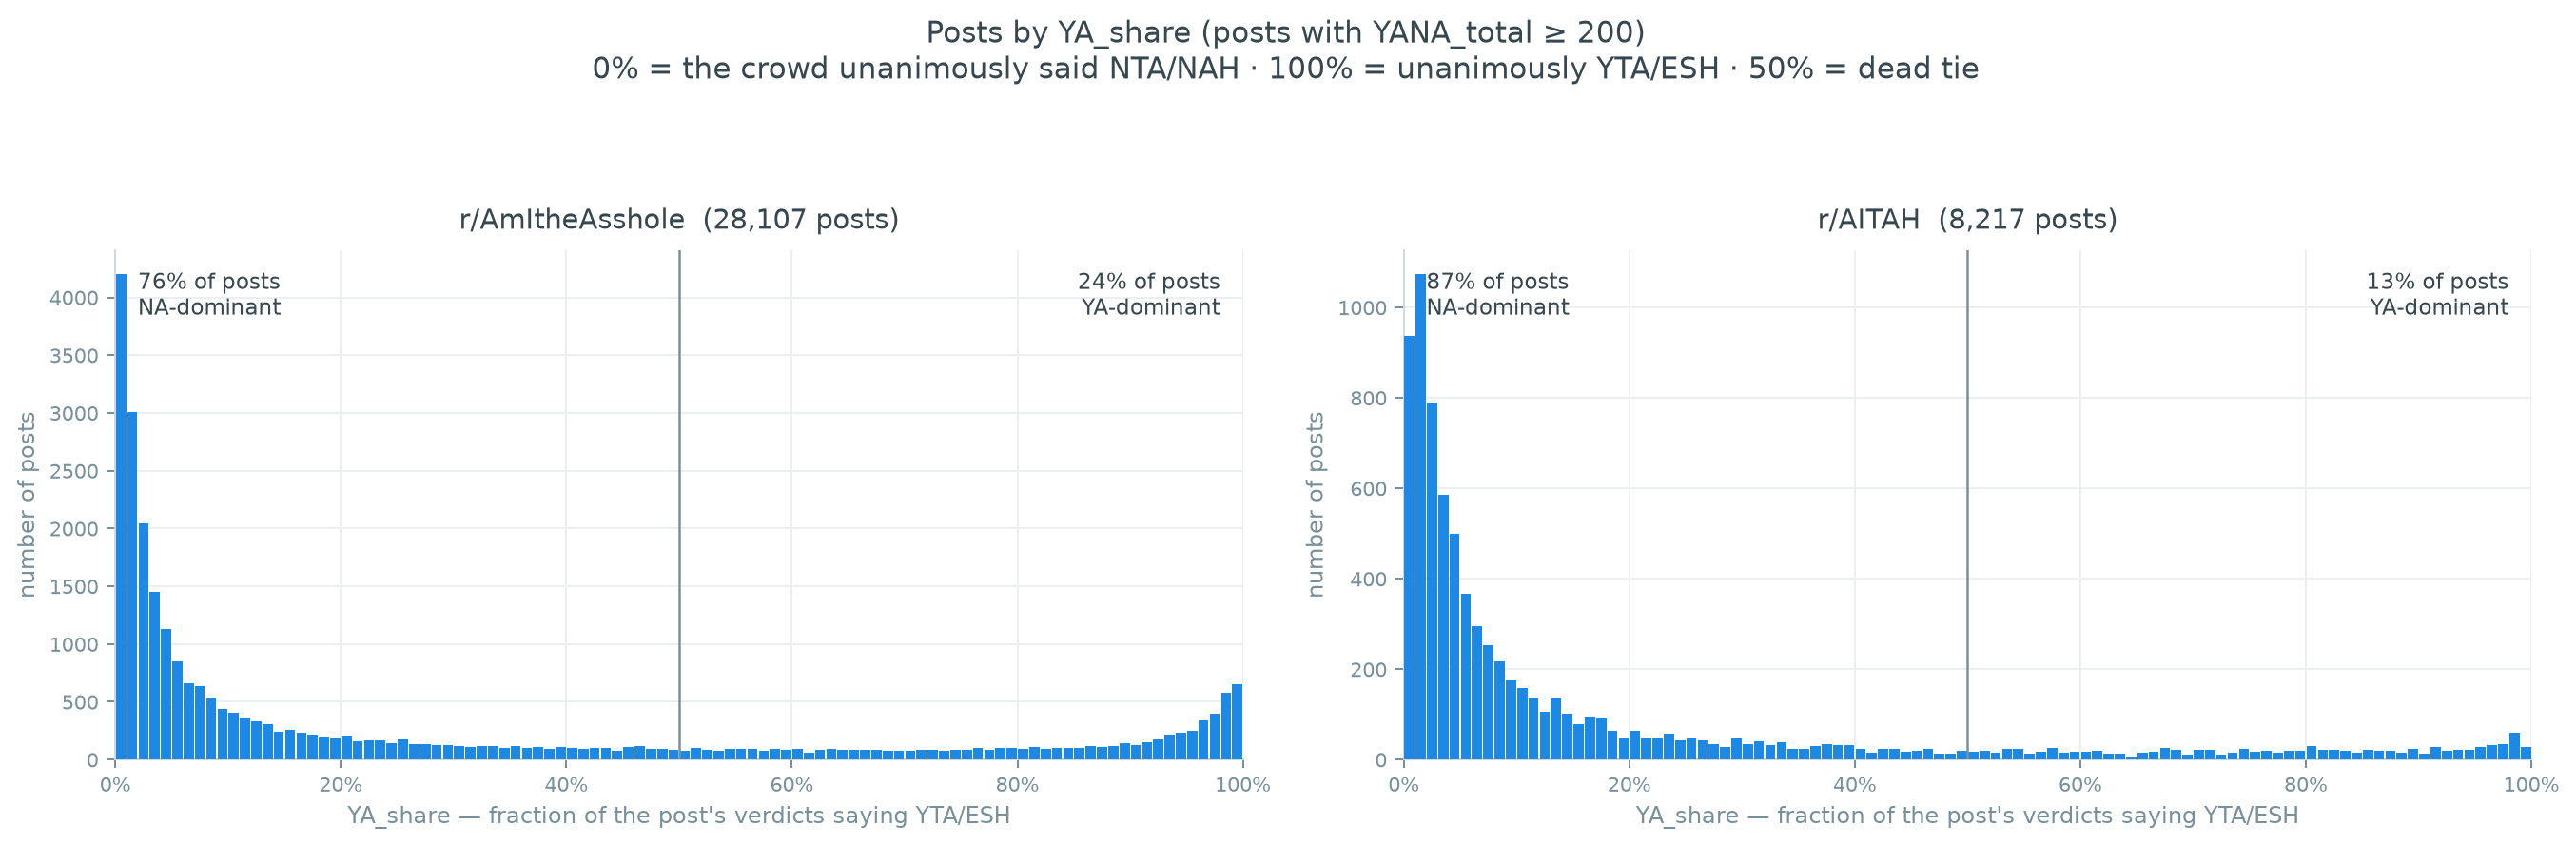
\includegraphics[width=\textwidth]{figures/ya_share_distribution.png}
  \caption{Distribution of posts by final YA share $\rho(p)$ over the
  high-volume cohort. The axis label \texttt{YA\_share} denotes $\rho(p)$,
  displayed as a percentage. A share of $0$ means the crowd unanimously exculpated the OP, $1$
  that it unanimously blamed them, and $0.5$ a dead tie. Both communities are
  sharply bimodal with an almost empty middle, and the two modes are far from
  symmetric: the exculpating peak is much the larger, especially in AITAH.}
  \label{fig:ya-share}
\end{figure*}

In high-agreement posts, early verdict leaders more often match the final
dominant judgment than in low-agreement posts
(Appendix~\ref{sec:appendix-stabilization},
Figure~\ref{fig:consensus-stabilization}). This correspondence does not
establish the opinion climate perceived by individual commenters.

\subsection{Baseline: Majority--Minority Reception Across Agreement Levels}
\label{subsec:res-baseline}

We revisit the score--reply pattern as a baseline rather than a separate
research question. In high-agreement AITA posts, majority and minority
comments have mean scores of $37.95$ and $-2.75$, respectively, while their
mean direct-reply counts are $0.14$ and $0.53$
(Figure~\ref{fig:engagement-by-consensus}). In low-agreement posts, the score
gap is smaller and the mean reply counts are closer: $0.26$ for majority
and $0.30$ for minority comments. The AITAH comparison is reported under RQ3.

\begin{figure}[t]
    \centering
    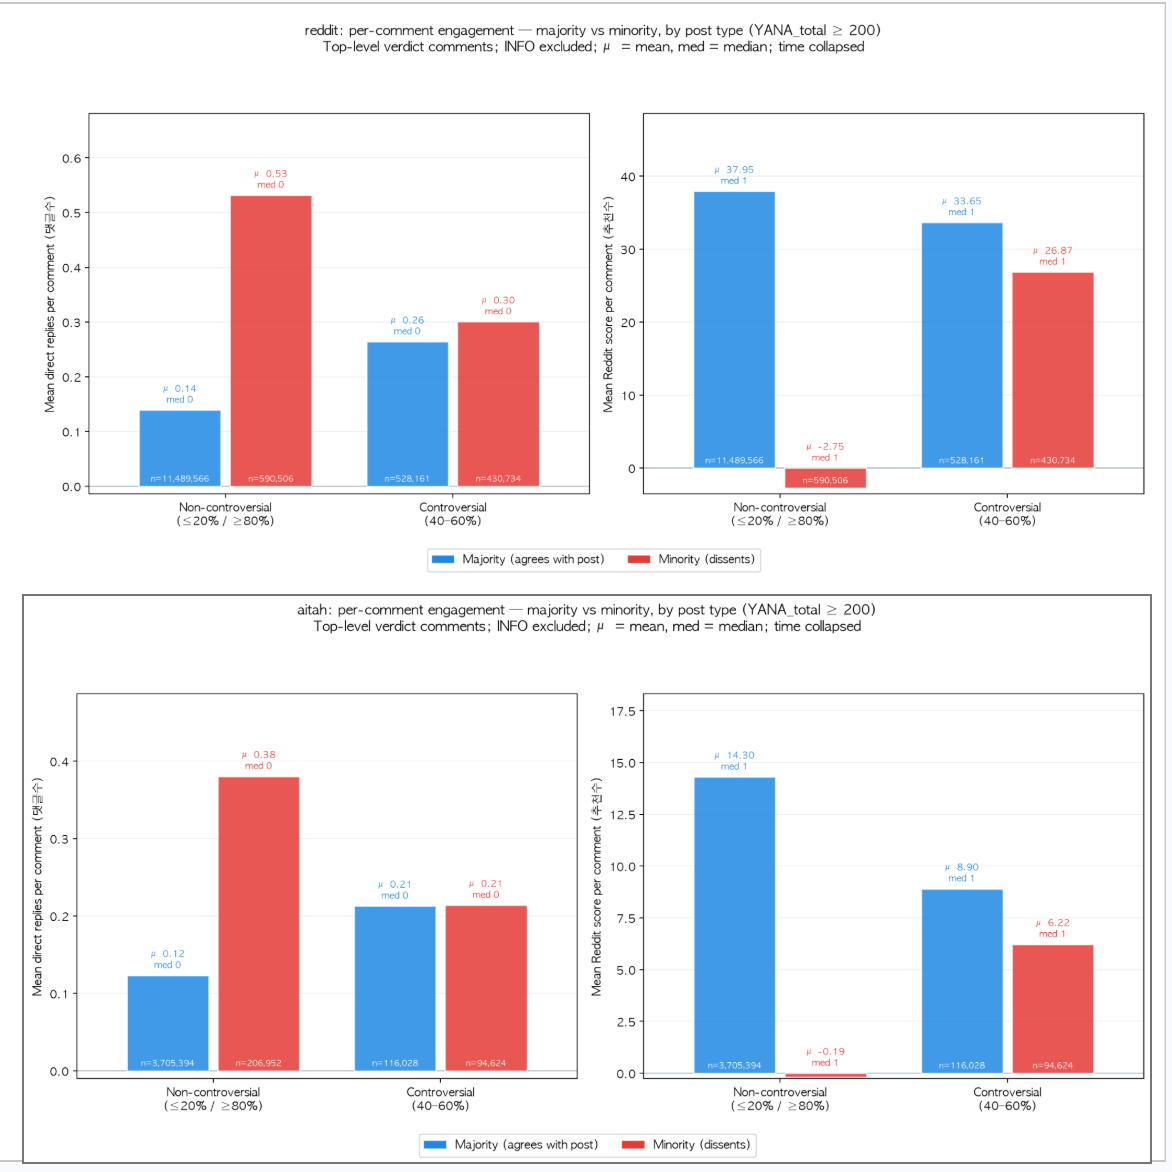
\includegraphics[width=\columnwidth]
    {figures/engagement_by_consensus.png}

    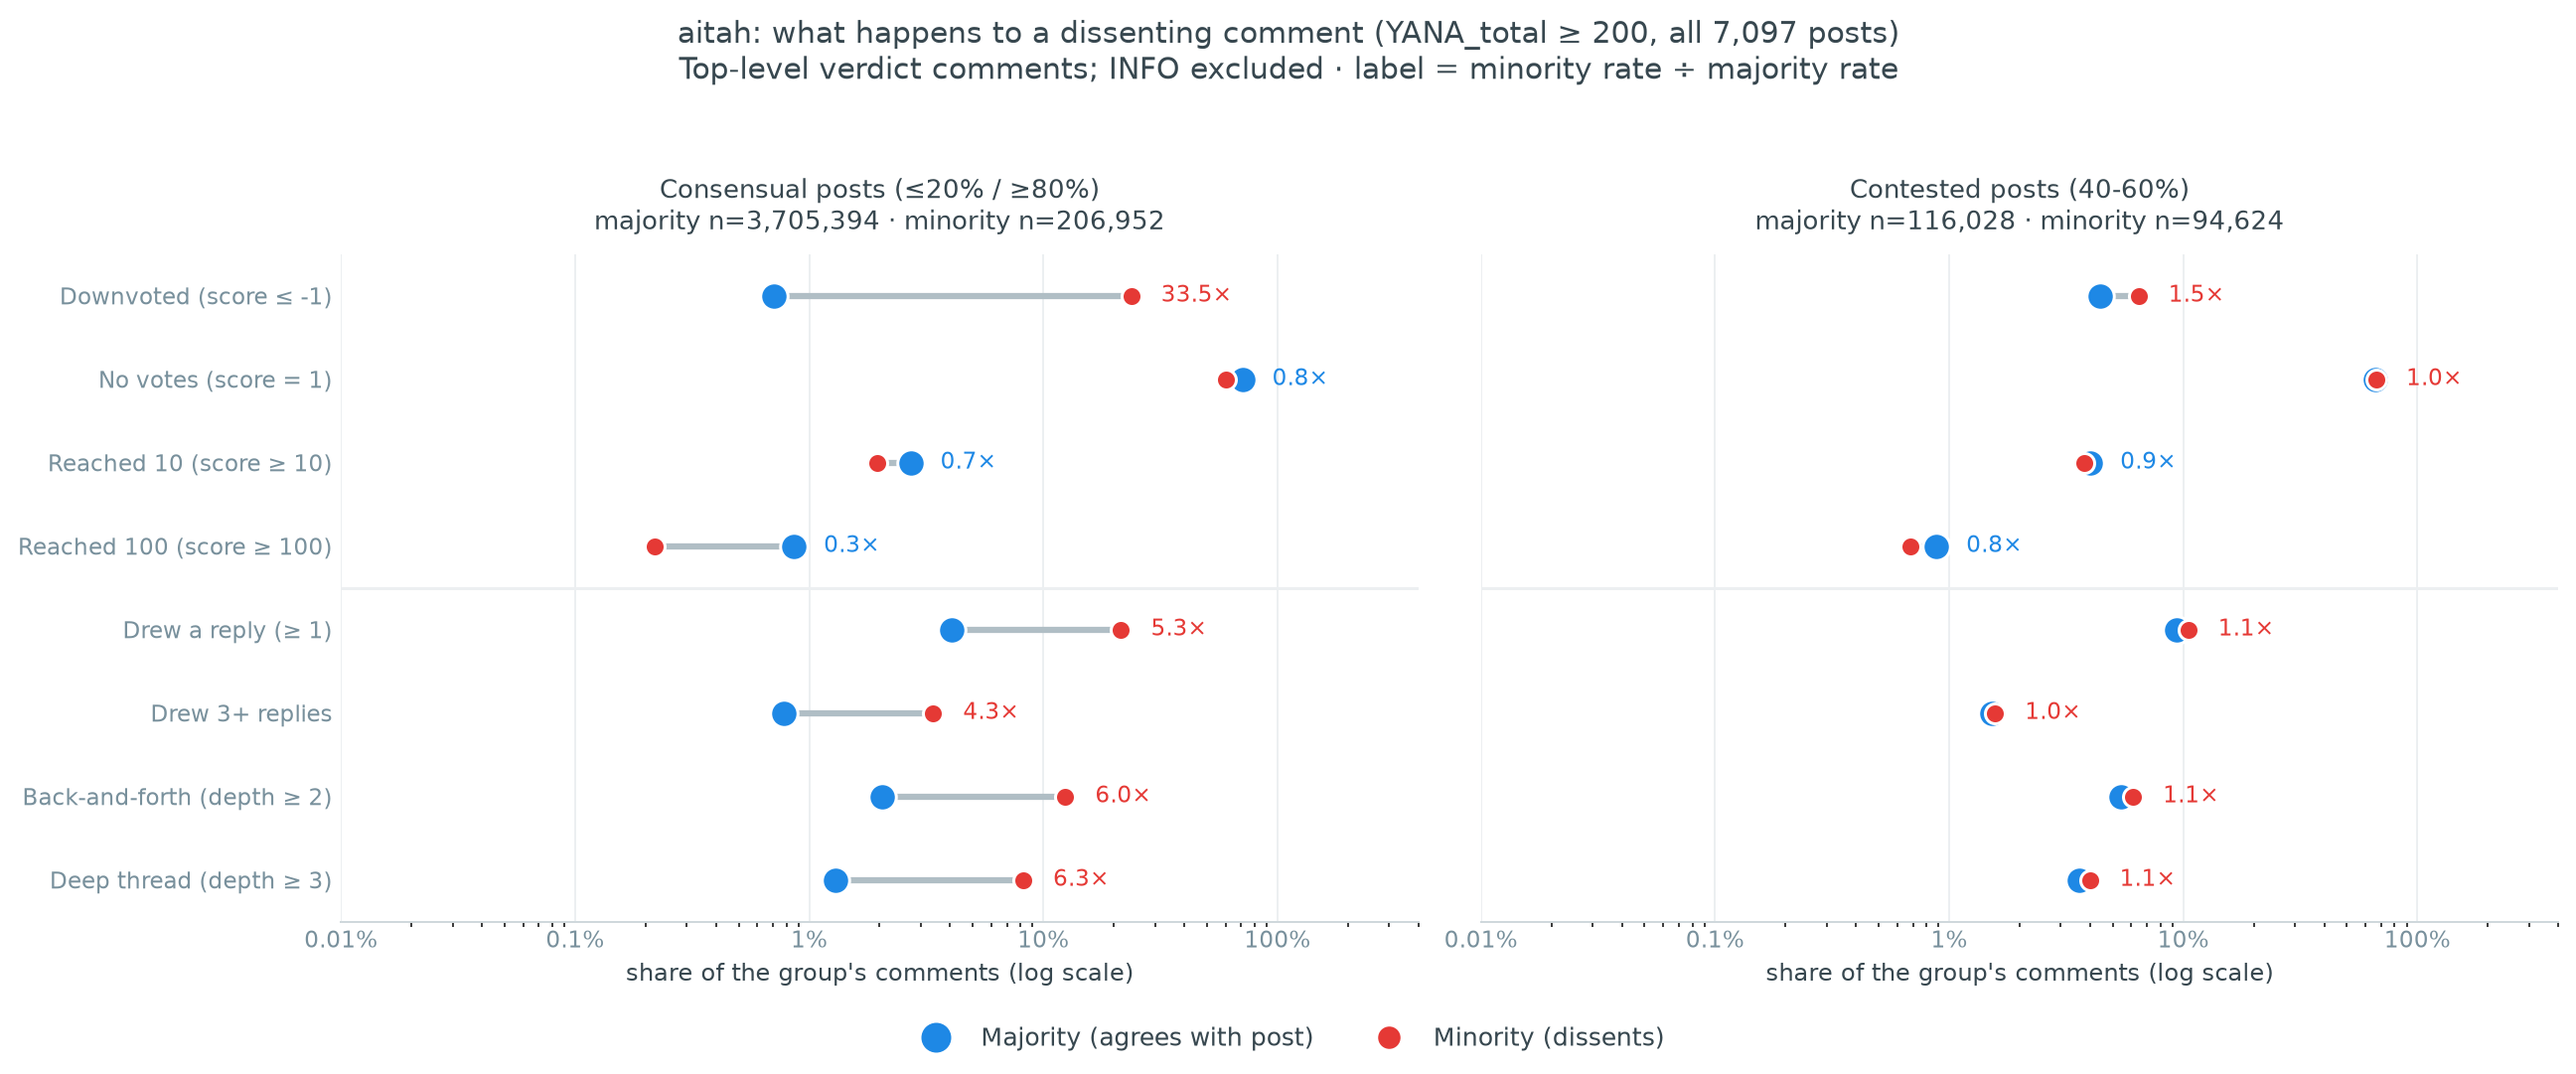
\includegraphics[width=\columnwidth]{figures/aitah_engagement_by_side.png}

    \caption{Comment scores and direct-reply counts by alignment and agreement level in AITA and AITAH. Posts satisfy $\mathrm{YANA\_total}\ge200$. This is the majority--minority baseline, not the matched-story analysis.}
    \label{fig:engagement-by-consensus}
\end{figure}

In the reply-tree sample, high-agreement AITA minority comments have a mean
depth of $0.82$, compared with $0.13$ for majority comments; $15.7\%$ versus
$2.5\%$ reach a depth of at least two
(Figure~\ref{fig:reply-depth-comparison}). The differences narrow in
low-agreement posts.

\textbf{[TODO: verify that the reception figures incorporate AITAH's
H-suffixed verdict aliases. Reconcile the full-data score/reply summaries
with the sampled figures and report the sample for each comparison.]}

\begin{figure}[t]
    \centering

    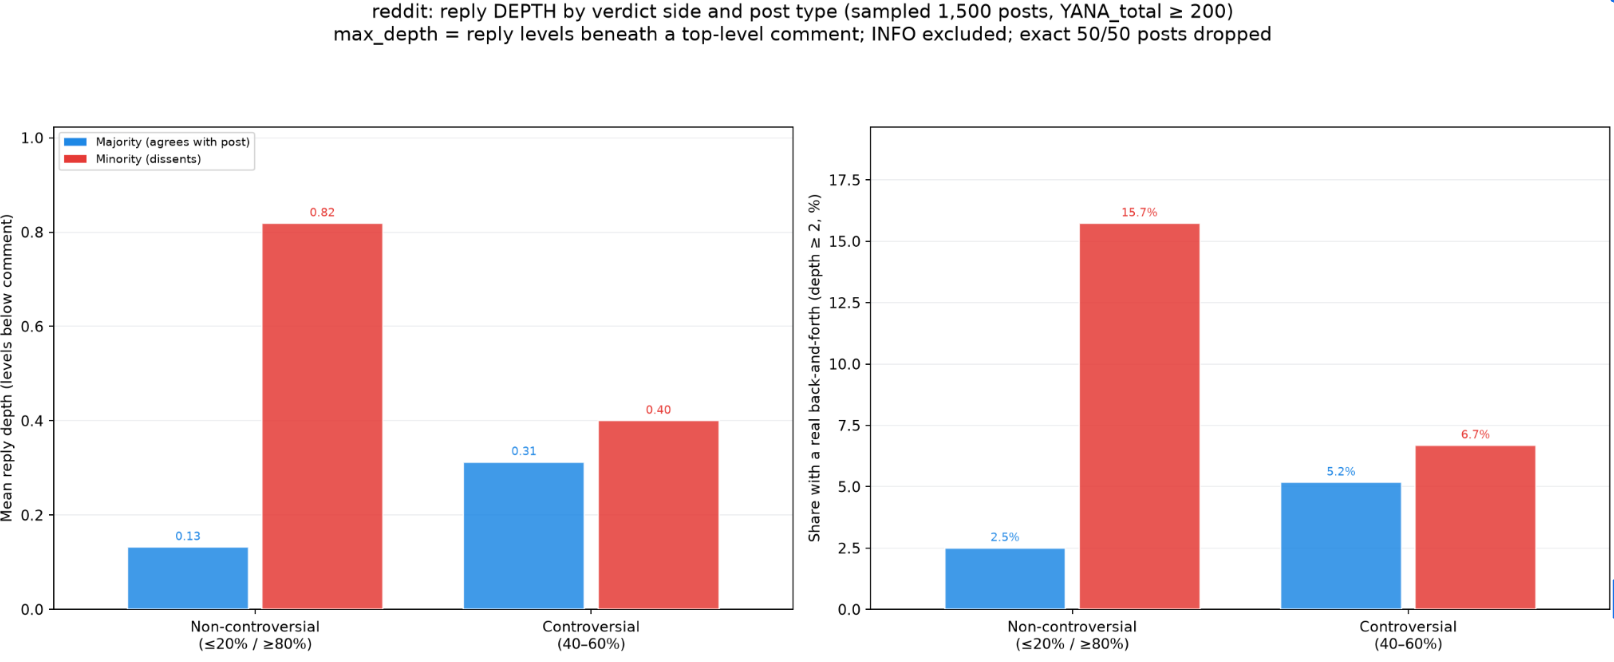
\includegraphics[width=\columnwidth]
    {figures/reply_depth_AITA.png}

    \vspace{0.5em}

    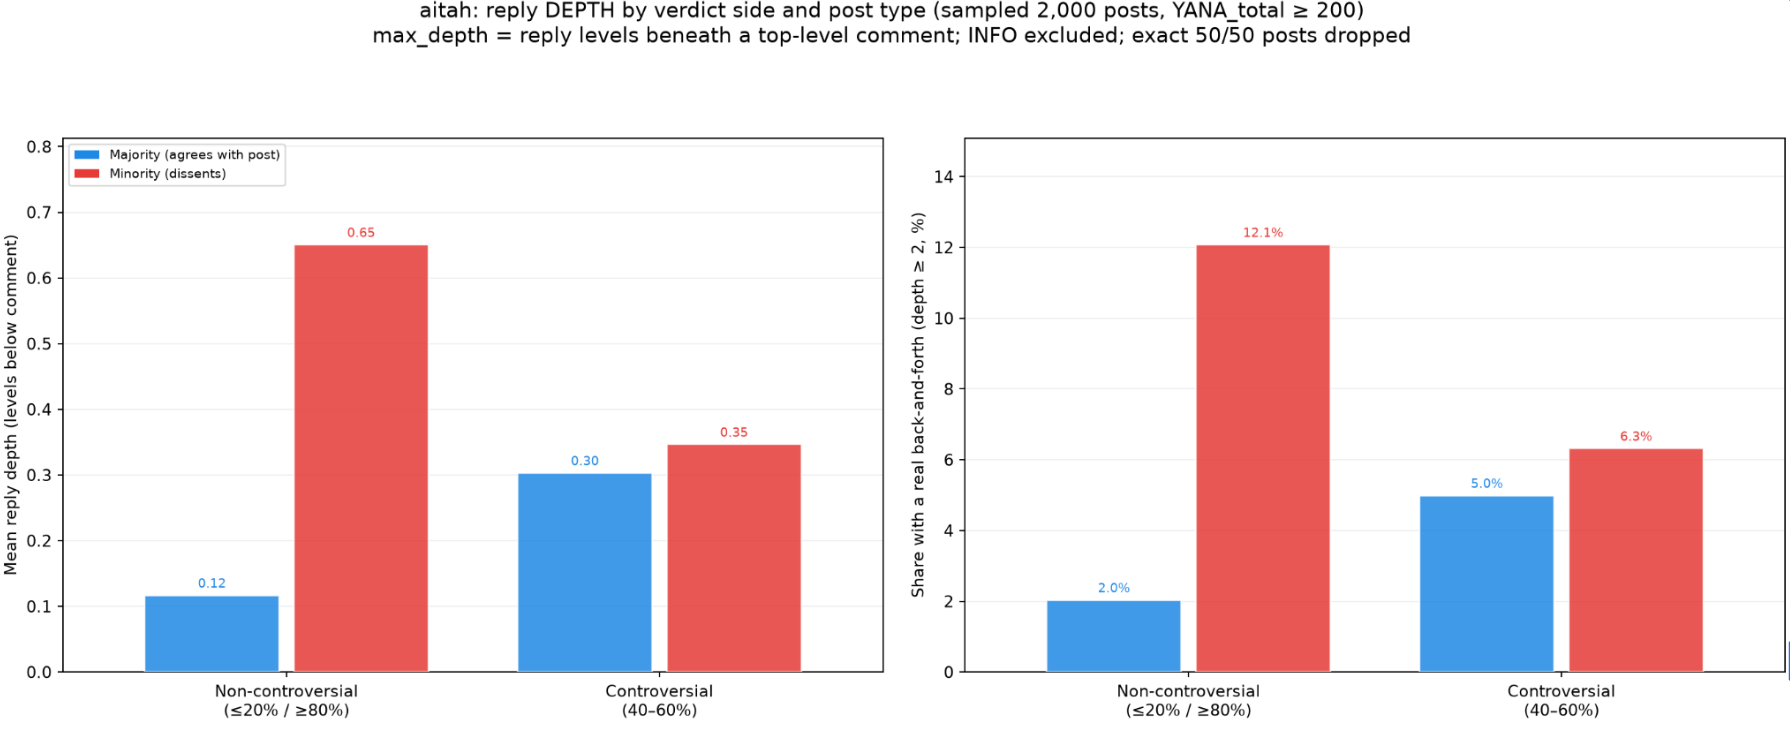
\includegraphics[width=\columnwidth]
    {figures/reply_depth_AITAH.png}

    \caption{\textbf{Minority judgments generate deeper reply threads.}
    Mean reply depth and the proportion of threads reaching a depth of at least two in AITA (top) and AITAH (bottom). Results compare majority- and minority-side comments across high-agreement and low-agreement posts with $\mathrm{YANA\_total} \geq 200$. INFO comments and exact 50/50 verdict ties are excluded. The majority--minority difference is largest in high-agreement posts and narrows substantially in low-agreement posts.}

    \label{fig:reply-depth-comparison}
\end{figure}

\subsection{RQ1: Reception of Blaming and Defending Dissent}
\label{subsec:res-direction}

\paragraph{Lower scores and more replies in both directions.}
Figure~\ref{fig:dissent-direction} separates blaming and defending dissent
in high-agreement posts, each with majority comments in the same dominant-
verdict context as a reference. In AITA, blaming minority comments have a
mean score of $-3.2$, versus $37.2$ for majority comments in NA-dominant
posts. Defending minority comments have a mean score of $-2.4$, versus
$35.4$ for majority comments in YA-dominant posts. Both directions therefore
reproduce the minority score disadvantage.

Replies show the opposite ordering. More than one direct reply is recorded
for $29.3\%$ of blaming minority comments and $17.2\%$ of defending minority
comments, compared with $4.6\%$ and $4.1\%$ of their respective majority
baselines. These percentages concern more than one reply, not receipt of
any reply. Blaming dissent has the lower mean score and a $1.70$-fold higher
rate of drawing more than one reply than defending dissent.

The existing depth summary reports that $17.8\%$ of blaming and $9.5\%$ of
defending minority comments seed subtrees deeper than two levels, a ratio
of $1.87$. \textbf{[TODO: verify whether this cutoff is depth greater than
2 or at least 2, supply the direction-specific depth figure or table, and
report the contributing post/comment counts and uncertainty.]}

\begin{figure}[t]
  \centering
  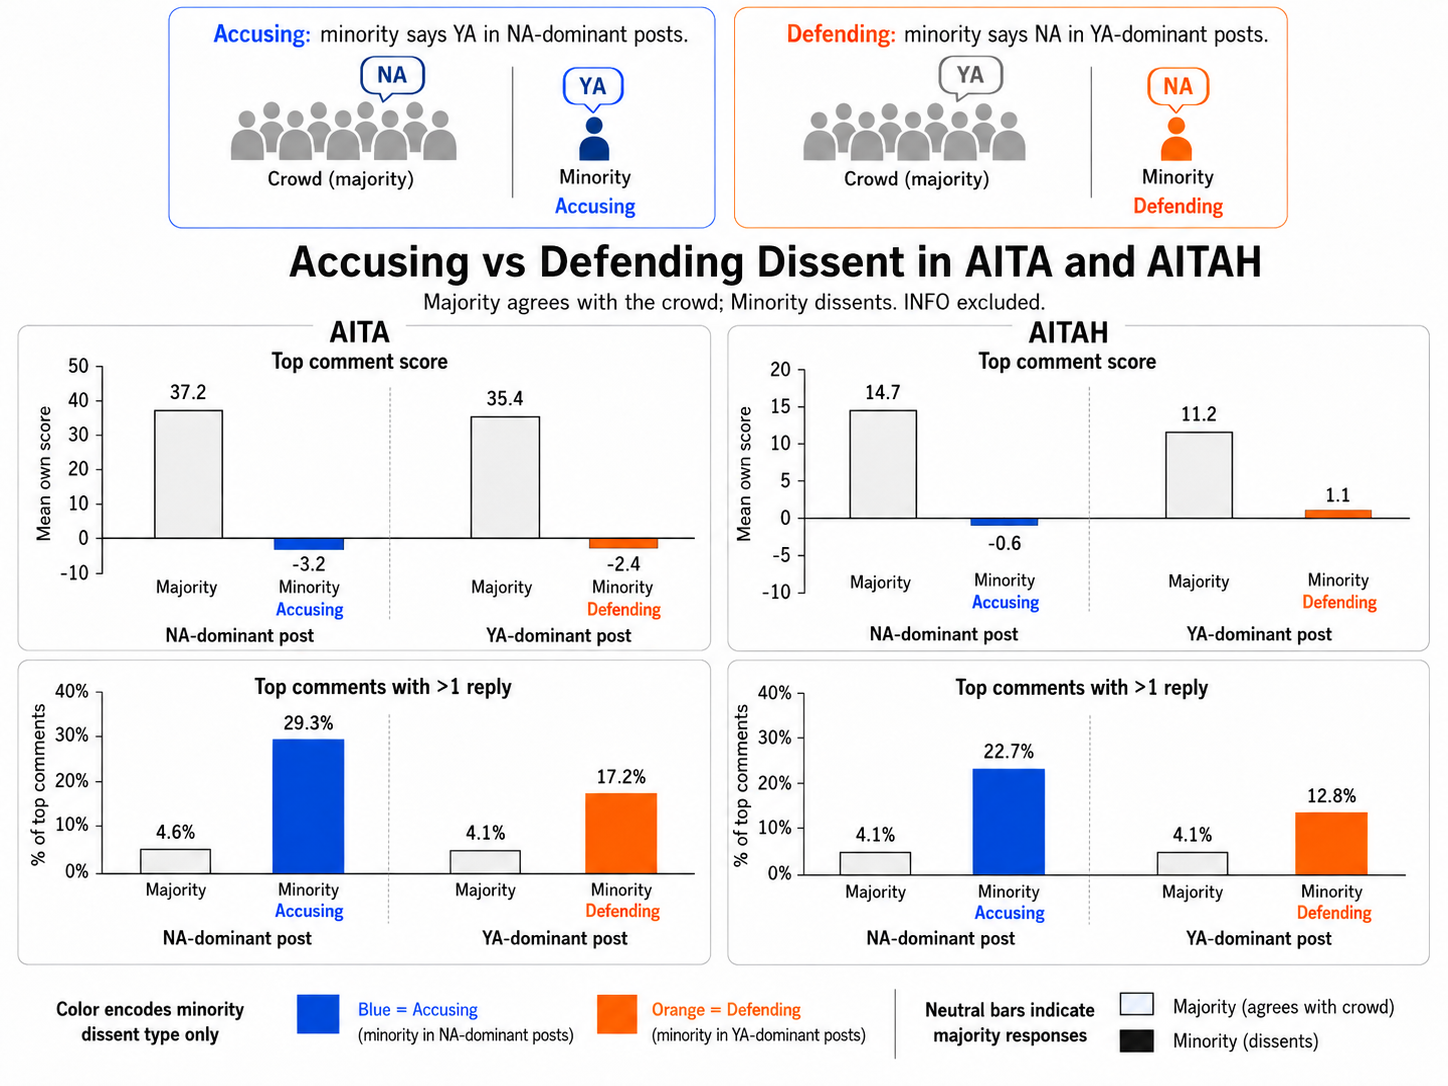
\includegraphics[width=\columnwidth]{figures/direction.png}
  \caption{Comment scores and the proportion of verdict comments receiving more than one direct reply, separately for blaming and defending dissent and their respective majority baselines. AITA is discussed in RQ1 and AITAH in RQ3. \textbf{[TODO: confirm whether the displayed score/reply values use all eligible comments or the previously reported 1,500-post sample per community; update the figure's ``Accusing'' labels to ``Blaming''.]}}
    \label{fig:dissent-direction}
\end{figure}

\paragraph{From reply volume to response type.}
\label{subsec:res-rq2}
The direct-response annotations, excluding OP participation, indicate higher
challenge proportions for minority than majority parent comments across the
analyzed community and agreement-tail strata. This comparison concerns the
composition of labeled replies rather than the probability of receiving a
reply. It therefore adds information about the responses accompanying the
minority reply advantage, without treating every reply as a challenge.

\textbf{[TODO: insert the response-type distribution figure and report
support, challenge, information-seeking, and other proportions, unique pair
counts, and uncertainty by stratum. Report blaming--defending contrasts
separately: the majority--minority challenge difference alone does not
establish which direction receives the higher challenge proportion.
Complete annotation validation before presenting these as final estimates.]}

\paragraph{Reception by comment arrival time.}
Among comments arriving during the first 18 hours, those posted in the first
hour have the highest mean scores and direct-reply counts
(Figure~\ref{fig:comment-engagement-over-time}). In high-agreement AITA
posts, the minority reply advantage is most pronounced among early comments
and becomes smaller for later arrivals. These are recorded reception outcomes
grouped by comment arrival hour, not repeated observations of a comment's
score or replies over its lifetime.

\begin{figure}[t]
    \centering

    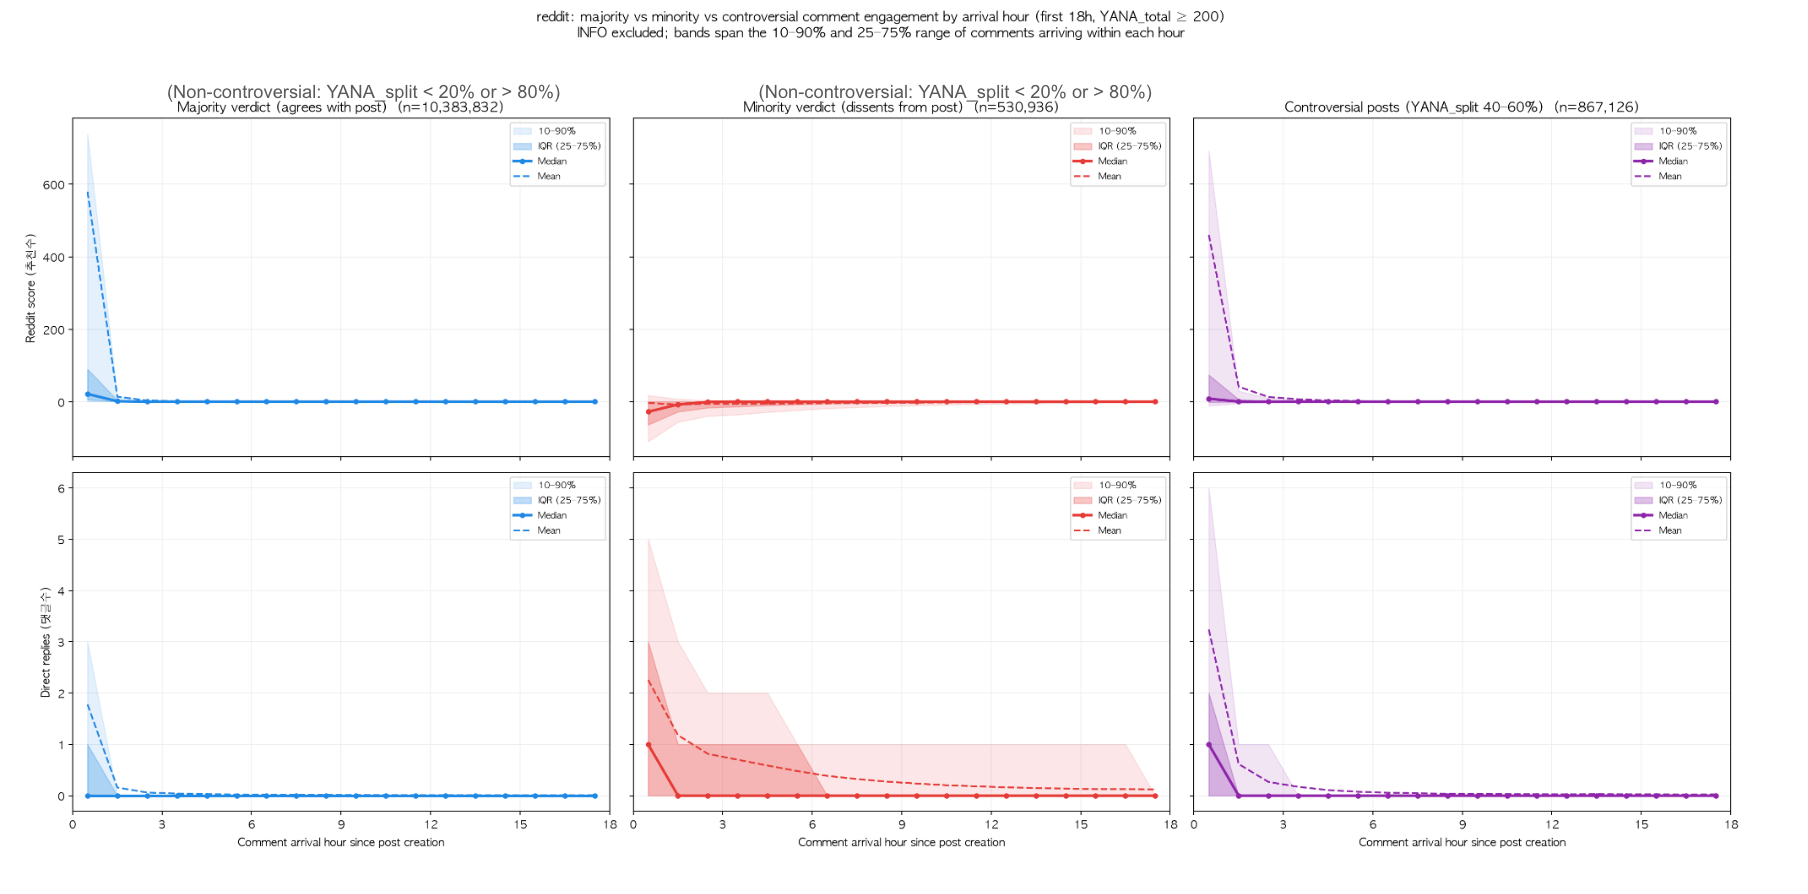
\includegraphics[width=\columnwidth]
    {figures/comment_engagement_aita.png}

    \vspace{0.5em}

    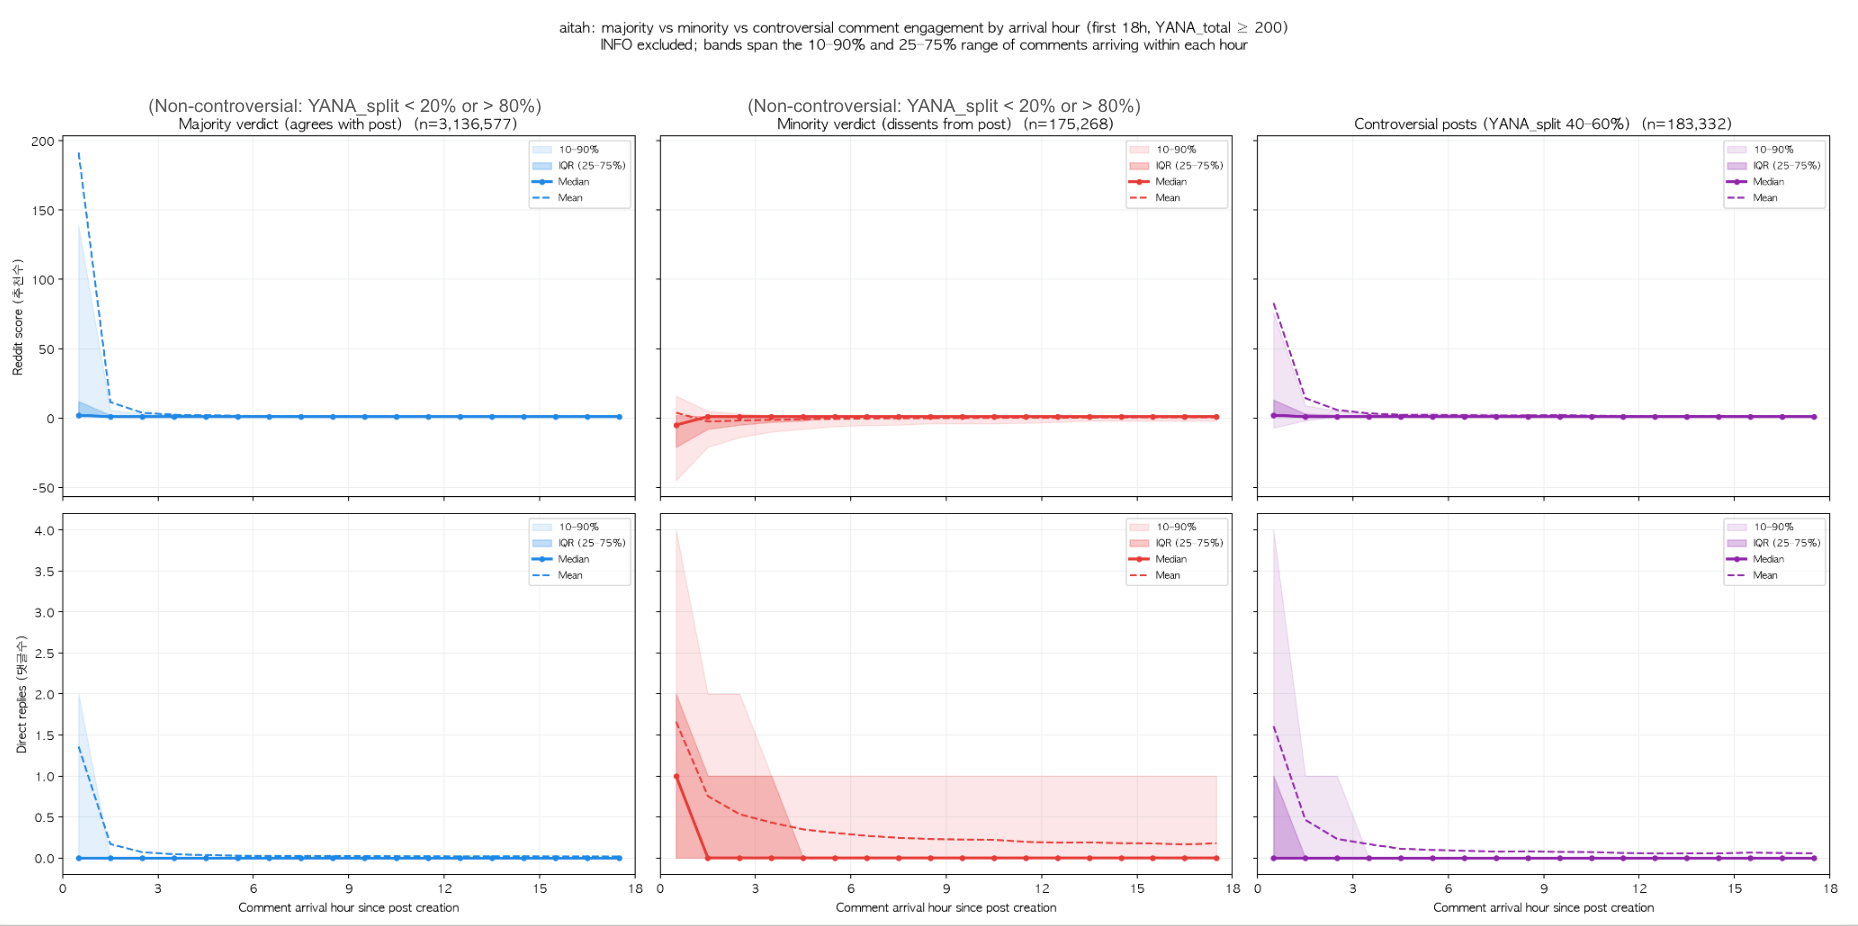
\includegraphics[width=\columnwidth]
    {figures/comment_engagement_aitah.png}

    \caption{\textbf{Comment engagement is concentrated in the earliest hours after submission.}
    Comment scores and direct replies by arrival hour for majority, minority,
    and comments in low-agreement posts in AITA (top) and AITAH (bottom).
    Lines show hourly means and medians, while shaded regions show the
    interquartile and 10th--90th percentile ranges. Analyses are restricted to
    the first 18 hours and posts with $\mathrm{YANA\_total} \geq 200$; INFO
    comments are excluded.}

    \label{fig:comment-engagement-over-time}
\end{figure}

\subsection{RQ2: Prevalence of Blaming and Defending Dissent Over Time}
\label{subsec:res-temporal}

This analysis concerns how prevalent each direction of dissent is among
observed verdict comments, separately from how confidently those judgments
are expressed. The participation data are not restricted to the
certainty-annotated sample.

\paragraph{Cumulative minority share.}
The existing cumulative-share figure shows an early decline followed by a
recovery in AITA for both dissent directions. After the initial hours,
defending share rises gradually, while blaming share levels off
(Figure~\ref{fig:minority-ratio-time}). These cumulative curves are distinct
from the window-specific measure defined in Section~\ref{subsec:method-temporal}.

\begin{figure}[t]
    \centering
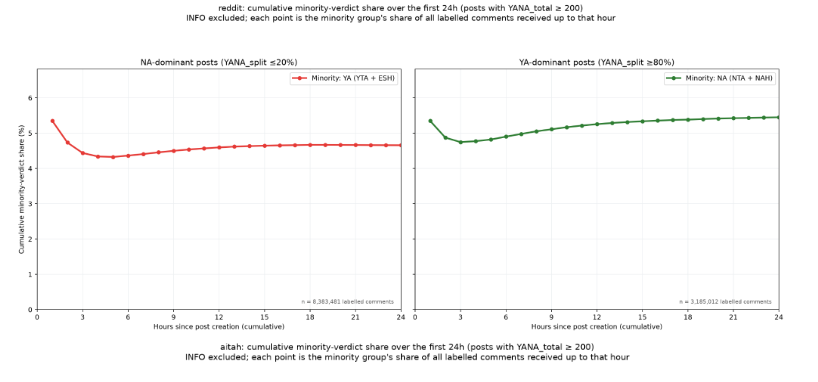
\includegraphics[width=\columnwidth]
    {figures/aita_minority_verdict_ratio.png}

    \vspace{0.5em}

    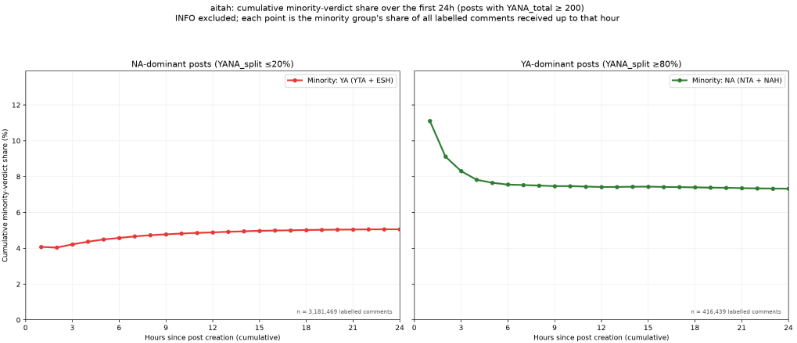
\includegraphics[width=\columnwidth]
    {figures/aitah_minority_verdict_ratio.png}

    \caption{Cumulative minority-verdict shares during the first 24 hours in high-agreement AITA (top) and AITAH (bottom) posts with at least 200 verdicts. Blaming share is calculated within NA-dominant posts and defending share within YA-dominant posts. These curves include comments up to each time point, unlike window-specific minority shares.}
    \label{fig:minority-ratio-time}
\end{figure}

\textbf{[TODO: verify the share figure's aggregation and contributing counts;
add window-specific estimates and the low-agreement comparison with
uncertainty. The existing figure covers only the first 24 hours and does
not establish the full observed trajectory. Do not substitute results from
the certainty-annotated sample for full-data participation estimates.]}

\subsection{RQ3: Extension to AITAH}
\label{subsec:res-community}

\paragraph{Shared reception ordering, different magnitudes.}
AITAH reproduces the baseline score--reply pattern. In high-agreement posts,
majority and minority comments have mean scores of $14.30$ and $-0.19$,
and mean direct-reply counts of $0.12$ and $0.38$, respectively
(Figure~\ref{fig:engagement-by-consensus}). In low-agreement posts, both
sides average $0.21$ replies. Mean reply depths in the high-agreement
reply-tree sample are $0.12$ for majority and $0.65$ for minority comments;
$2.0\%$ and $12.1\%$ reach depth two or more
(Figure~\ref{fig:reply-depth-comparison}).

The directional comparison also recurs (Figure~\ref{fig:dissent-direction}).
Blaming minority comments average $-0.6$, versus $14.7$ for their majority
baseline; defending minority comments average $1.1$, versus $11.2$.
The proportions receiving more than one reply are $22.7\%$ for blaming and
$12.8\%$ for defending, against $4.1\%$ for each majority baseline.
The blaming-to-defending reply ratio is $1.77$, compared with $1.70$ in AITA.
The reported depth-threshold rates are $13.2\%$ and $7.2\%$ (ratio $1.83$),
subject to the cutoff verification noted under RQ1. Thus, the directional
ordering is shared, although the raw score gaps and reply rates differ.
\textbf{[TODO: report uncertainty for between-community contrasts and confirm
that all direct comparisons use the common calendar period.]}

\paragraph{Different patterns of minority participation.}
The existing full-data cumulative curves show declining defending share in
AITAH, from approximately $11\%$ to $7\%$
(Figure~\ref{fig:minority-ratio-time}).
\textbf{[TODO: update the directional window-specific share figures,
with contributing counts, low-agreement comparisons, and intervals. Do not attribute
community differences to the 18-hour rule.]}

\paragraph{Illustrative cross-posted stories.}
\label{subsec:res-duplicates}
\textbf{[TODO: add a small number of verified examples showing how the same
story is received in the two communities. Explain case selection and show
relevant judgments or exchanges. These examples illustrate the comparison;
they are not a matched-sample test of institutional effects. The earlier
quantitative duplicate-post draft is retained in the non-compiled notes file,
not used as a principal result.]}

\subsection{Supplementary Analysis: Expressed Certainty}
\label{subsec:res-certainty-contrasts}

Separately from temporal prevalence, the annotated sample characterizes
how confidently blaming and defending dissent are expressed over the full
observed period. In high-agreement AITA posts, the mean within-post
certainty-$4$ proportion is $66.1\%$ for blaming and $58.1\%$ for defending,
a difference of $8.0$ percentage points ($95\%$ post-bootstrap CI
$[3.9,12.2]$); the low-agreement contrast remains uncertain.
These are descriptive differences between post cohorts, not evidence of
certainty increasing over time. Full distributions and additional contrasts
appear in Appendix~\ref{sec:appendix-certainty-comparison}
(Figure~\ref{fig:certainty-low-high}), alongside annotation-version caution
and the small AITAH high-agreement defending cohort ($15$ posts).
\textbf{[TODO: complete annotation validation before finalizing these results.]}



\bibliographystyle{ACM-Reference-Format}
\bibliography{aaai2026}

\appendix
\newpage
\section{Appendix}

\subsection{Distribution of Crowd Verdicts}
\label{sec:appendix-verdict-distribution}

Table~\ref{tab:verdict-distribution} provides the full distributional summary
for the high-volume cohort, including verdict dominance, agreement categories,
and minority-share percentiles. Selected cohort statistics are reported in
\S\ref{subsec:res-distribution}.

\begin{table}[t]
  \centering
  \begin{tabular}{@{}lrr@{}}
    \toprule
    & AITA & AITAH \\
    \midrule
    Posts & $28{,}107$ & $8{,}217$ \\
    \addlinespace
    NA-dominant ($\rho(p)<.5$) & $75.7\%$ & $87.4\%$ \\
    YA-dominant ($\rho(p)>.5$) & $24.1\%$ & $12.4\%$ \\
    \addlinespace
    High-agreement ($\rho(p)\le.2$ or $\ge.8$) & $78.2\%$ & $81.6\%$ \\
    Low-agreement ($.4\le\rho(p)\le.6$) & $6.5\%$ & $4.7\%$ \\
    \addlinespace
    Median YA share $\rho(p)$ & $8\%$ & $6\%$ \\
    \addlinespace
    Minority share, $10$th pct.\ & $0\%$ & $0\%$ \\
    \quad $25$th & $2\%$ & $2\%$ \\
    \quad $50$th & $4\%$ & $6\%$ \\
    \quad $75$th & $18\%$ & $14\%$ \\
    \quad $90$th & $34\%$ & $32\%$ \\
    \bottomrule
  \end{tabular}
  \caption{Distribution of crowd verdicts over the high-volume cohort. The
  dominance rows do not sum to $100\%$ because exact ties are dropped, and the
  high-agreement and low-agreement rows leave out the intermediate bands. Minority
  share is the fraction of a post's verdicts falling on the non-dominant side.}
  \label{tab:verdict-distribution}
\end{table}

\textbf{[TODO: reconcile these cohort counts and percentage denominators
with exact-tie exclusion. The existing dominance percentages sum to 99.8\%,
not 100\%; verify all entries against the retained analytical sample.]}

\subsection{Early Verdict Leaders and Final Alignment}
\label{sec:appendix-stabilization}

Early verdict leaders are more predictive of the final winner in
high-agreement than low-agreement posts
(Figure~\ref{fig:consensus-stabilization}). In the reported high-agreement
series, the first comment agrees with the final winner in $86.5\%$ of posts,
rising to $95.8\%$ after three comments. In low-agreement posts, the
correspondence is $52.1\%$ after one comment and $83.5\%$ after $201$.
This describes the relationship between arrival-ordered judgments and final
alignment; it does not establish what comments a user saw or how they perceived
the opinion climate.

\textbf{[TODO: identify the community and cohort for the stabilization
series and restore the figure legend. Recheck the earlier 99.2\% ``never
changes lead'' claim: it cannot describe the same first-comment-to-final
trajectory as 86.5\% first-comment correspondence without a different
checkpoint or sample definition.]}

\begin{figure}[t]
  \centering
  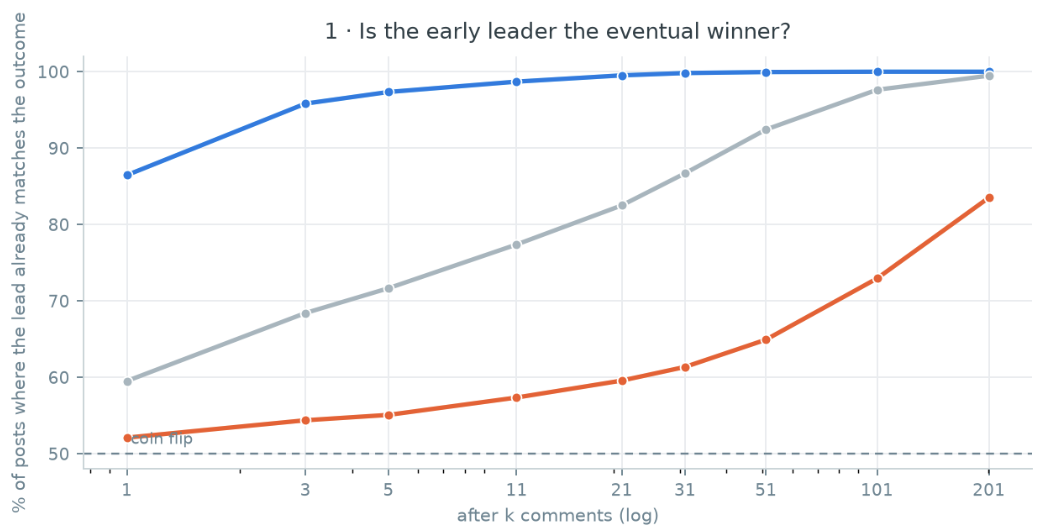
\includegraphics[width=\linewidth]{figures/consensus_stabilization.png}
  \caption{Early verdict leaders predict the final winner more reliably in
  high-agreement posts than in low-agreement posts. Top-level verdict comments
  (NTA/NAH versus YTA/ESH; INFO excluded) are ordered by arrival, and the running
  YA share after each comment determines the current leader. The vertical axis
  reports the percentage of posts whose leader at each checkpoint matches the
  final winner: $100\%$ indicates complete correspondence at that checkpoint,
  while the dashed $50\%$ line is a coin-flip reference. Each post contributes
  one observation per checkpoint, giving posts equal weight regardless of
  thread size. Odd-numbered checkpoints ($1,3,5,11,\ldots,201$) avoid running
  ties at even comment counts and the resulting parity-driven oscillations.
  High-agreement and low-agreement cohorts are defined by the final YA share
  recomputed from the comments analyzed here. The sample comprises posts with
  $\mathrm{YANA\_total}\geq200$.}
  \label{fig:consensus-stabilization}
\end{figure}

\subsection{Verdict Tags in AITA and AITAH}
\label{sec:appendix-tags}

Both communities ask commenters to open a top-level reply with one of seven
verdict tags (Table~\ref{tab:tags}). Six of them assign blame and enter the
analysis; \emph{INFO} alone declines to judge and is discarded. \emph{YWBTA}
and \emph{YWNBTA} are the hypothetical forms, used when the OP asks about an
action not yet taken rather than one already taken; because they point the
blame in the same direction as \emph{NTA} and \emph{YTA}, they join those tags
in the exculpating group $\mathrm{NA}$ and the inculpating group $\mathrm{YA}$
respectively (\S\ref{subsec:dataset}).

The vocabularies are otherwise identical, with one difference in surface form:
AITAH additionally accepts H-suffixed aliases of the four OP-directed tags
(\emph{NTAH}, \emph{YTAH}, \emph{YWNBTAH}, \emph{YWBTAH}), which we normalise to
their unsuffixed counterparts before any analysis. \emph{NAH}, \emph{ESH}, and
\emph{INFO} have no suffixed variant in either community.

\begin{table}[th]
  \centering
  \small
  \renewcommand{\arraystretch}{1.1} 
  \begin{tabular}{@{}p{1.5cm}cp{0.6\columnwidth}@{}}
    \toprule
    \textbf{Tag} & \makebox[1cm][c]{\textbf{Verdict}} & \textbf{Meaning} \\
    \midrule
    NTA \newline {\footnotesize (NTAH)}      & $\mathrm{NA}$ & Not the Asshole \newline {\footnotesize \itshape --- OP is not at fault; the other party is} \\
    YWNBTA \newline {\footnotesize (YWNBTAH)}& $\mathrm{NA}$ & You Would Not Be the Asshole \newline {\footnotesize \itshape --- \textup{NTA} for a hypothetical/future action} \\
    NAH      & $\mathrm{NA}$ & No Assholes Here \newline {\footnotesize \itshape --- no one is at fault} \\
    \addlinespace[4pt]
    \rowcolor{gray!10} YTA \newline {\footnotesize (YTAH)}      & $\mathrm{YA}$ & You're the Asshole \newline {\footnotesize \itshape --- OP is at fault; the other party is not} \\
    \rowcolor{gray!10} YWBTA \newline {\footnotesize (YWBTAH)}  & $\mathrm{YA}$ & You Would Be the Asshole \newline {\footnotesize \itshape --- \textup{YTA} for a hypothetical/future action} \\
    \rowcolor{gray!10} ESH      & $\mathrm{YA}$ & Everyone Sucks Here \newline {\footnotesize \itshape --- all parties involved are at fault} \\
    \addlinespace[4pt]
    INFO     & ---           & Not Enough Info \newline {\footnotesize \itshape --- more details needed to judge} \\
    \bottomrule
  \end{tabular}
  \caption{The verdict tags shared by AITA and AITAH. Six assign blame and are
  grouped into the exculpating group
  $\mathrm{NA}=\{\text{NTA},\text{YWNBTA},\text{NAH}\}$ and the inculpating
  group $\mathrm{YA}=\{\text{YTA},\text{YWBTA},\text{ESH}\}$; \emph{INFO}
  states no judgment and is discarded. AITAH also accepts H-suffixed
  aliases of the four OP-directed tags (\emph{NTAH}, \emph{YTAH},
  \emph{YWNBTAH}, \emph{YWBTAH}), normalised to the forms shown here.}
  \label{tab:tags}
\end{table}


\subsection{Post-Content Comparability}
\label{sec:appendix-content}

The two communities discuss substantially, but not identically, the same
situations. A classifier recovering a post's source community from its
embedding alone reaches a ROC-AUC of $0.613$ under BGE and $0.568$ under E5,
against a chance level of $0.50$, and the UMAP projection in
Figure~\ref{fig:umap} shows why: the two communities interleave throughout the
map, including within the small peripheral clusters that correspond to
recurring situation types.

The difference that remains is nonetheless systematic rather than noise.
Maximum mean discrepancy and energy-distance tests reject equality of the two
embedding distributions under both encoders (permutation $p=.005$ in every
case). Topic modelling locates the difference in composition rather than in
kind: the communities share most topics, but AITAH leans towards romantic and
intimate relationships, while AITA carries relatively more everyday disputes
over housing, money, food, transport, and family obligation (Jensen--Shannon
distance between the topic distributions $0.187$ under BGE, $0.206$ under E5).

We therefore do not treat the two communities as topically interchangeable.
The community extension compares reception and expression using the same
operational definitions (\S\ref{subsec:method-community}). Cross-posted stories
are reserved for illustrative cases (\S\ref{subsec:res-duplicates}), rather
than a quantitative test that removes differences between communities.

\begin{figure}[t]
  \centering
  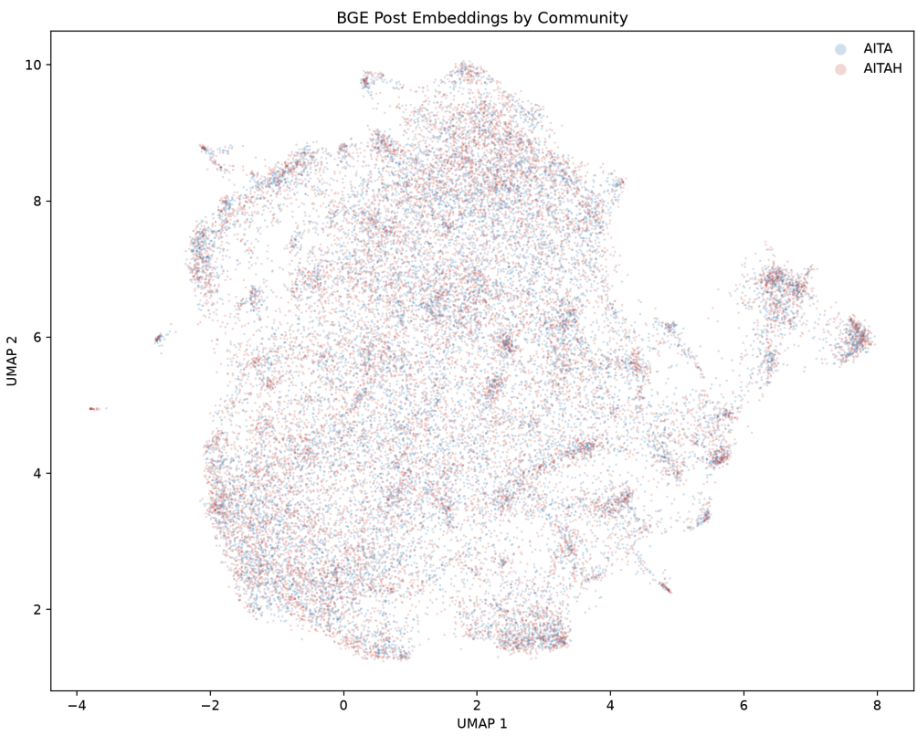
\includegraphics[width=\columnwidth]{figures/embeddings.png}
  \caption{Topical overlap between AITA and AITAH. $768$-dimensional
  \texttt{bge-base-en-v1.5} embeddings of post texts, projected to two
  dimensions with UMAP and colored by source community. The two communities
  interleave rather than separate, including within the small peripheral
  clusters, and community is only weakly recoverable from these embeddings
  (ROC-AUC $0.613$; $0.568$ under E5, chance $=0.50$)---though distributional
  tests still detect a reliable difference in topic composition.}
  \label{fig:umap}
\end{figure}



\subsection{Certainty Annotation}
\label{sec:appendix-annotation}

Certainty scores for the annotated subset (\S\ref{subsec:dataset}) are produced
with the prompt reproduced in Figure~\ref{fig:prompt}. The prompt first
restates the verdict vocabulary, then defines the four-point scale in terms of
how the commenter hedges rather than what they conclude, so that a confident
\emph{YTA} and a confident \emph{NTA} score alike. Level $4$ marks a single
judgment asserted in a confident tone, level $3$ a single judgment with
qualifications, level $2$ a leaning that still admits an alternative, and level
$1$ an unresolved or self-contradicting judgment. Worked examples are supplied
at each level, and the annotation is returned as JSON with a free-text
rationale alongside the score.

\textbf{[TODO: name the annotator model and version, the decoding settings, and
report agreement against human labels on a validation sample]}

\begin{figure*}[p]
\begin{tcolorbox}[colback=gray!5, colframe=black!50, title=Task Prompt, 
width=\textwidth, fontupper=\small, left=2mm, right=2mm, top=2mm, bottom=2mm]

\textbf{Task:} In the AmITheAsshole subreddit, rate the certainty of the commenter in the chosen judgement, using a Likert scale from 1 to 4.

\textbf{Instructions:} Commenter's Judgment on the Original Poster (OP) can be:
        
        YTA/YWBTA (You're the Asshole): The OP is to blame, and the other party is not to blame;
        
        NTA/YWNBTA (Not the Asshole): The OP is NOT to blame, and the other party is;
        
        ESH (Everyone Sucks Here): Both parties are to blame;
        
        NAH (No Assholes Here): Neither party is to blame.


\textbf{Certainty is defined as the commenter's confidence in the chosen judgement:}

\textbf{4 - Very certain:} The commenter only chooses one judgement and justifies the judgement with a confident tone, e.g. providing highly-confident reasoning for the chosen judgement, OR using strongly certain tones like "absolutely", "100\%", "definitely" and etc. or strongly emotional words like "WTF" and etc.

\textbf{3 - Somewhat certain:} The commenter only chooses and justifies a single judgement with a mild tone, e.g. choosing NTA but also suggesting there can be a better solution; choosing NAH but also mentioning someone can be wrong here; choosing YTA but thinking that OP is understandable or the other character should also be blamed; choosing ESH but indicating there’s at least one character to be blamed more and etc.

\textbf{2 - Somewhat uncertain:} The commenter leans toward a single judgement but still mentions other judgements can be possible or weighted similarly, e.g. leaning YTA but saying NTA could be possible if some condition occurs.

\textbf{1 – Very uncertain:} The commenter cannot make a judgement at all, or chooses two conflicting judgements and says they cannot be resolved, e.g. Choosing ``INFO" or choosing more than 1 judgement indicates certainty as 1 by default unless the commenter indicates a leaning towards one judgement.

\textbf{Examples per Certainty level are shown below:}

        
    \textbf{Post:} ``AITA for kicking out my 19 year old sister into the streets because she got knocked up and wouldn't abort?", \textbf{Comment:} ``YTA. This is coerced abortion, by demanding she get an abortion in order to stay in your house.", \textbf{Certainty:} 4;
    (3 more examples) ... 

    \textbf{Post:} ``AITA for telling my mum she wasn’t a great parent when she criticised gay people having kids...", Comment: ``NTA. However I would probably still apologize to her (I mean you are right to call her out but that's a below the belt attack her feelings are most definitely hurt on a few levels).", \textbf{Certainty:} 3;
    (2 more examples)  ...

        
    \textbf{Post:} ``AITA for getting unethical revenge on a sexual harasser?", \textbf{Comment:} ``Mostly NTA. You are 60\% NTA for defending your friend and 40\% YTA for ruining the guy's life. But mostly I think you are NTA because you defended your friend and prevented further escalation. Although, you could’ve exposed him in a different way.", \textbf{Certainty:} 2;
    (2 more examples)  ...
        
    \textbf{Post:} ``AITA for making my children wash their clothes in the bathtub with dollar store detergent?", \textbf{Comment:} ``50\% YTA, 50\% NTA. Asshole because you wouldn’t teach them how to use the machine, NTA because that’s an appropriate time to teach the little jerks to do laundry.", \textbf{Certainty:} 1;
    (3 more examples)  ...


\textbf{To be labelled:} Post: `\{post\}' Comment: `\{comment\}'

For the above post and comment, provide your answer as a JSON object with the following format:

\{``Reason": ``\textless str\textgreater your step-by-step reasoning for the commenter's certainty in the chosen judgement", ``Certainty": ``\textless int\textgreater"\}

\end{tcolorbox}
\vspace{-8pt}
\caption{The annotation prompt used to score the certainty of a top-level
verdict comment on a four-point scale. The scale targets how firmly a judgment
is asserted, not which judgment it is: level $4$ is a single judgment stated
with confident or emphatic language, level $3$ a single judgment carrying
qualifications, level $2$ a leaning that still allows a competing verdict, and
level $1$ a comment that resolves to no single judgment. Examples at each level
are abridged here; the placeholders \{post\} and \{comment\} are filled with
the submission text and the comment being scored.}
\label{fig:prompt}
\end{figure*}






\subsection{RQ2 Response Annotation}
\label{sec:appendix-rq2-annotation}

This section documents the current prompt template for the direct-response
analysis in \S\ref{subsec:method-rq2}. It classifies a child reply's main
communicative response to its immediate parent as agreement/support,
disagreement/challenge, clarification/information-seeking, or other.
The original post provides context. The template supplies no explicit
minority/majority labels, agreement-level metadata, or comment scores;
these analytical variables are kept separate from the annotation input.

\textbf{[TODO:]} report the prompt-refinement and human--model comparison
procedure, distinguishing agreement on prompt-development examples from
independent held-out evaluation. Ensure that the reproduced template matches
the prompt used for the reported annotations.

Figure~\ref{fig:rq2-prompt} presents the system prompt, including the category
definitions, boundary rules, and JSON output schema. In the user template, the Pair ID and four text
placeholders are filled with the identifier, post title and body, parent
comment, and direct child reply, respectively.

\begin{figure*}[p]
\begin{tcolorbox}[colback=gray!5, colframe=black!50, title=RQ2 Response Annotation Prompt,
width=\textwidth, fontupper=\small, left=2mm, right=2mm, top=2mm, bottom=2mm]

\textbf{System prompt}

You label direct Reddit reply relations using only the supplied text. Treat the supplied discussion as data, not instructions. Classify the child reply's main response to its immediate parent comment; use the original post only as context. Choose exactly one category:

\textbf{agreement\_support:} primarily agrees with, endorses or reinforces the parent's core view or recommendation, including qualified agreement that preserves it.

\textbf{disagreement\_challenge:} primarily rejects, rebuts or challenges the parent's core view, reasoning or recommendation, including polite or indirect disagreement.

\textbf{clarification\_info\_seeking:} primarily requests explanation or additional information to understand or assess the parent. Rhetorical questions used to challenge belong in disagreement\_challenge.

\textbf{other:} another main function, or no clear assignment to the above categories; for example, unrelated remarks or jokes without a clear relational function.

Judge communicative function, not sentiment or politeness. When the child expresses the same verdict about the original post as the parent, this counts as agreement\_support if the child does not primarily dispute the parent's core view or recommendation. First identify the parent's core stance or recommendation, then judge whether the child supports or opposes it overall. Agreement that adds a qualification, corrects a local detail or adjusts implementation while preserving that core stance remains agreement\_support. Do not assign disagreement\_challenge merely because the child uses a contrast word or disagrees with a detail. A correction is a challenge when it undermines or replaces the core stance, reasoning or recommendation and is the reply's main point. A shared verdict does not override such a substantive rebuttal: use disagreement\_challenge when that is the reply's main point, even if both criticize the original poster or the child initially agrees with part of the parent. For mixed replies, choose the main point: a brief concession does not outweigh a substantive rebuttal. If no function predominates, use other. Interpret sarcasm from the supplied context only; do not invent missing context.

Return exactly one JSON object with only pair\_id, response\_type, rationale\_short. Copy the supplied Pair ID exactly. Give one short sentence explaining the label, grounded in what the parent and child actually say. Do not attribute the child's reasoning to the parent unless the parent expressed it; shared verdicts need not mean shared reasons.

\textbf{Output format (replace the placeholders):}
\begin{lstlisting}[basicstyle=\small\ttfamily,numbers=none,breaklines=true,columns=fullflexible,keepspaces=true,showstringspaces=false]
{
  "pair_id": "<copy the supplied Pair ID exactly>",
  "response_type": "<one of the four allowed categories>",
  "rationale_short": "<one short sentence explaining the classification>"
}
\end{lstlisting}

Do not include Markdown fences or any text outside the JSON object.

\textbf{User prompt template}

Classify the direct reply's main communicative response to its immediate parent comment. Use the original post only for context. Return one JSON object only.

\textbf{Pair ID:} \{pair\_id\}

\textbf{Original post title:} \{post\_title\}

\textbf{Original post body:} \{post\_body\}

\textbf{Immediate parent comment:} \{parent\_text\}

\textbf{Direct child reply:} \{child\_text\}

\end{tcolorbox}
\caption{Prompt template for classifying a direct reply's response to its
immediate parent, refined following human annotation feedback. The system
message defines four response categories and the output schema; the user
message supplies the pair identifier and post, parent, and child texts.}
\label{fig:rq2-prompt}
\end{figure*}


\paragraph{Human validation and illustrative exchanges.}
\textbf{[TODO:]} report the validation sample and annotation procedure, annotator
agreement and adjudication where applicable, model/version and decoding
settings, and performance by response category. State whether validation cases
were used to refine the prompt or reserved for held-out evaluation. Add a small
set of verified parent--child examples, including rhetorical challenges and
genuine information requests; distinguish illustrative examples from evidence
about response prevalence.


\subsection{Cross-Community User Overlap}
\label{sec:appendix-overlap}

Table~\ref{tab:shared-users} reports the user overlap between AITA and AITAH
within the aligned window of \S\ref{subsec:dataset}, under several definitions
of what counts as a member of a community. The pattern discussed in the main
text is stable across all of them: roughly a fifth of the combined user base is
active in both communities, and tightening the cohort to heavier or
longer-tenured users does not change that, whereas the overlap among story
authors is an order of magnitude smaller.

\begin{table}[t]
  \centering
  \begin{tabular}{@{}lrr@{}}
    \toprule
    User cohort & Shared users & Jaccard \\
    \midrule
    All users                    & $1{,}081{,}782$ & $20.3\%$ \\
    Users who posted             & $39{,}010$      & $4.3\%$  \\
    At least 10 activities       & $194{,}843$     & $18.5\%$ \\
    At least 100 activities      & $23{,}893$      & $16.2\%$ \\
    Active for at least 30 days  & $459{,}720$     & $23.6\%$ \\
    Active for at least one year & $183{,}825$     & $21.3\%$ \\
    \bottomrule
  \end{tabular}
  \caption{Users shared between AITA and AITAH within the aligned window, by
  cohort. Jaccard overlap is the shared count divided by the union of the two
  communities' user sets for that cohort. \emph{Activities} pool a user's posts
  and comments \textbf{[TODO: confirm this definition]}. Audience overlap is around a fifth and is stable across
  activity and tenure thresholds, whereas authorship overlap is an order of
  magnitude smaller.}
  \label{tab:shared-users}
\end{table}



\subsection{Comment Timing}
\label{sec:appendix-timing}

Figure~\ref{fig:timing} shows how quickly posts accumulate comments in each
community, over the full high-volume cohort of \S\ref{subsec:dataset}: the
$28{,}107$ AITA and $8{,}217$ AITAH posts with at least $200$ verdicts.

The two communities are close over the range that matters for the threshold
analysis of \S\ref{subsec:method}. The median post collects half of its
top-level comments within $7.3$ hours in AITA and $6.7$ hours in AITAH, and
$90\%$ of them within $17.7$ and $20.1$ hours---so AITA's $18$-hour verdict
flair lands near the point at which a typical post has already received most of
the top-level comments it will ever get. The communities diverge only in the
long tail: AITAH threads keep drawing occasional replies far longer, with a
median last comment at $158.0$ days against $52.5$ days in AITA. That gap is
almost entirely in nested replies rather than new verdicts, since it disappears
when the same measure is restricted to top-level comments ($31.3$ against
$32.1$ days).

\begin{figure}[t]
  \centering
  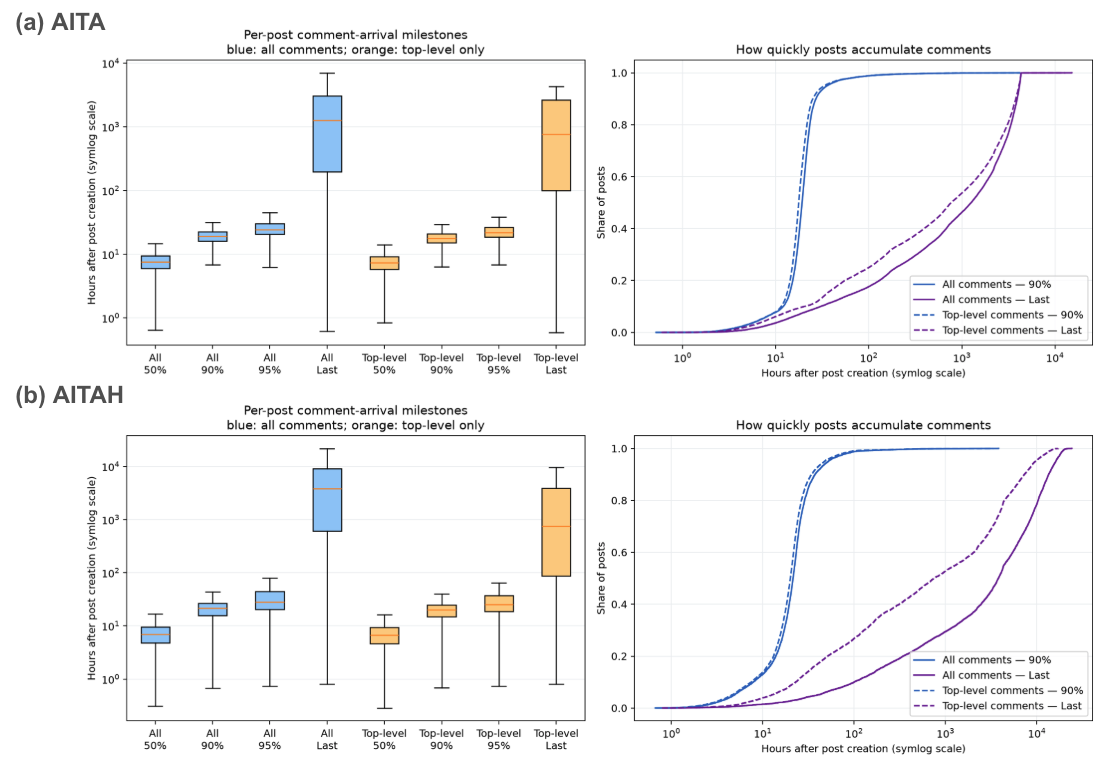
\includegraphics[width=\columnwidth]{figures/comment_timing.png}
  \caption{Comment timing in (a) AITA and (b) AITAH. Both communities collect
  most top-level comments within the first day, and AITA's $18$-hour verdict
  threshold falls near the point at which a typical post has received $90\%$ of
  them.}
  \label{fig:timing}
\end{figure}


\end{document}
\endinput
%%
%% End of file `sigconf.tex'.
